\documentclass[12pt,a4paper]{report}

% Packages
\usepackage[utf8]{inputenc}
\usepackage[T1]{fontenc}
\usepackage{geometry}
\usepackage{graphicx}
\usepackage{listings}
\usepackage{xcolor}
\usepackage{hyperref}
\usepackage{titlesec}
\usepackage{parskip}
\usepackage{caption}
\usepackage{float}

% Page margins
\geometry{a4paper, top=1.6cm, bottom=1.6cm, left=2.5cm, right=2.5cm}

\usepackage{booktabs}
\usepackage{array}


% Hyperref setup
\hypersetup{
    colorlinks=true,
    linkcolor=black,
    urlcolor=black,
}

% Remove "Chapter X" prefix from chapter headings
\titleformat{\chapter}[block]
  {\normalfont\LARGE\bfseries}  % format
  {}                             % label (empty = no "Chapter X")
  {0pt}                          % sep
  {\LARGE\bfseries}              % before-code

\titlespacing*{\chapter}{0pt}{-20pt}{20pt}

% ─────────────────────────────────────────────
\begin{document}

% ── Title Page ───────────────────────────────
\begin{titlepage}
    \centering
    \vspace*{\fill}
    {\LARGE\bfseries Pattern Recognition \\ Assignment \#1\par}
    \vspace{2cm}
    {\LARGE  \quad \textit{Diabetes Risk Prediction} \par}
    \vspace*{\fill}
\end{titlepage}

% ── Table of Contents ───────────────────────
\tableofcontents
\newpage

% ── Introduction ───────────────────────────
\chapter{Introduction}
\Large This Lab Assignment Focuses on Machine Learning Concepts in multiclass classification. \\
It envolve the implementation of the following algorithms:
\begin{itemize}
    \item K-Nearest Neighbors (KNN)
    \item Softmax Regression
    \item Neural Networks
\end{itemize}
The Challenge is to Balance the dataset and to achieve the best possible performance in predicting diabetes risk. \\ \\
The report is structured as follows:
\begin{itemize}
    \item Chapter 2: Data Preprocessing
    \item Chapter 3: K-Nearest Neighbors (KNN)
    \item Chapter 4: Softmax Regression
    \item Chapter 5: Neural Networks
    \item Chapter 6: Evaluation Metrics
\end{itemize}

\newpage

% ── Data Preprocessing ─────────────────────
\chapter{Data Preprocessing}
\section{Overview}
\Large In this chapter, we will discuss the steps taken to preprocess the diabetes dataset.\\
The sequence of steps was as follows:
\begin{enumerate}
    \item Duplicates Removal
    \item Data Correlation Analysis
    \item Feature Selection
    \item Data Splitting
    \item Data Balancing
    \item Data Normalization
\end{enumerate}

\newpage
\section{Data Correlation Analysis}
\begin{figure}[H]
    \hspace{-2.7cm}
    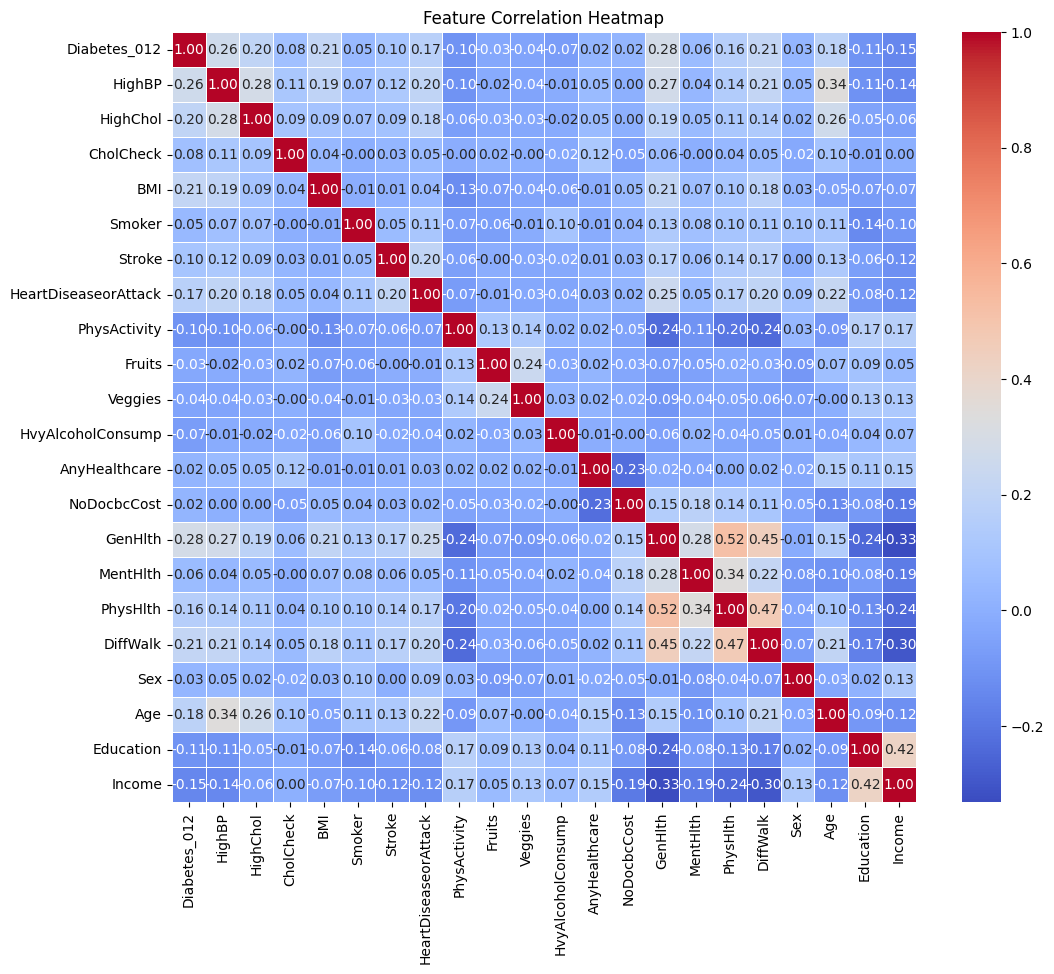
\includegraphics[width=1.3\textwidth]{datapreprocessing/data-correlation.png}
    \caption{Correlation Heatmap of the Diabetes Dataset}
\end{figure}

\newpage
\section{Feature Selection}
\begin{figure}[H]
    \hspace{-1.5cm}
    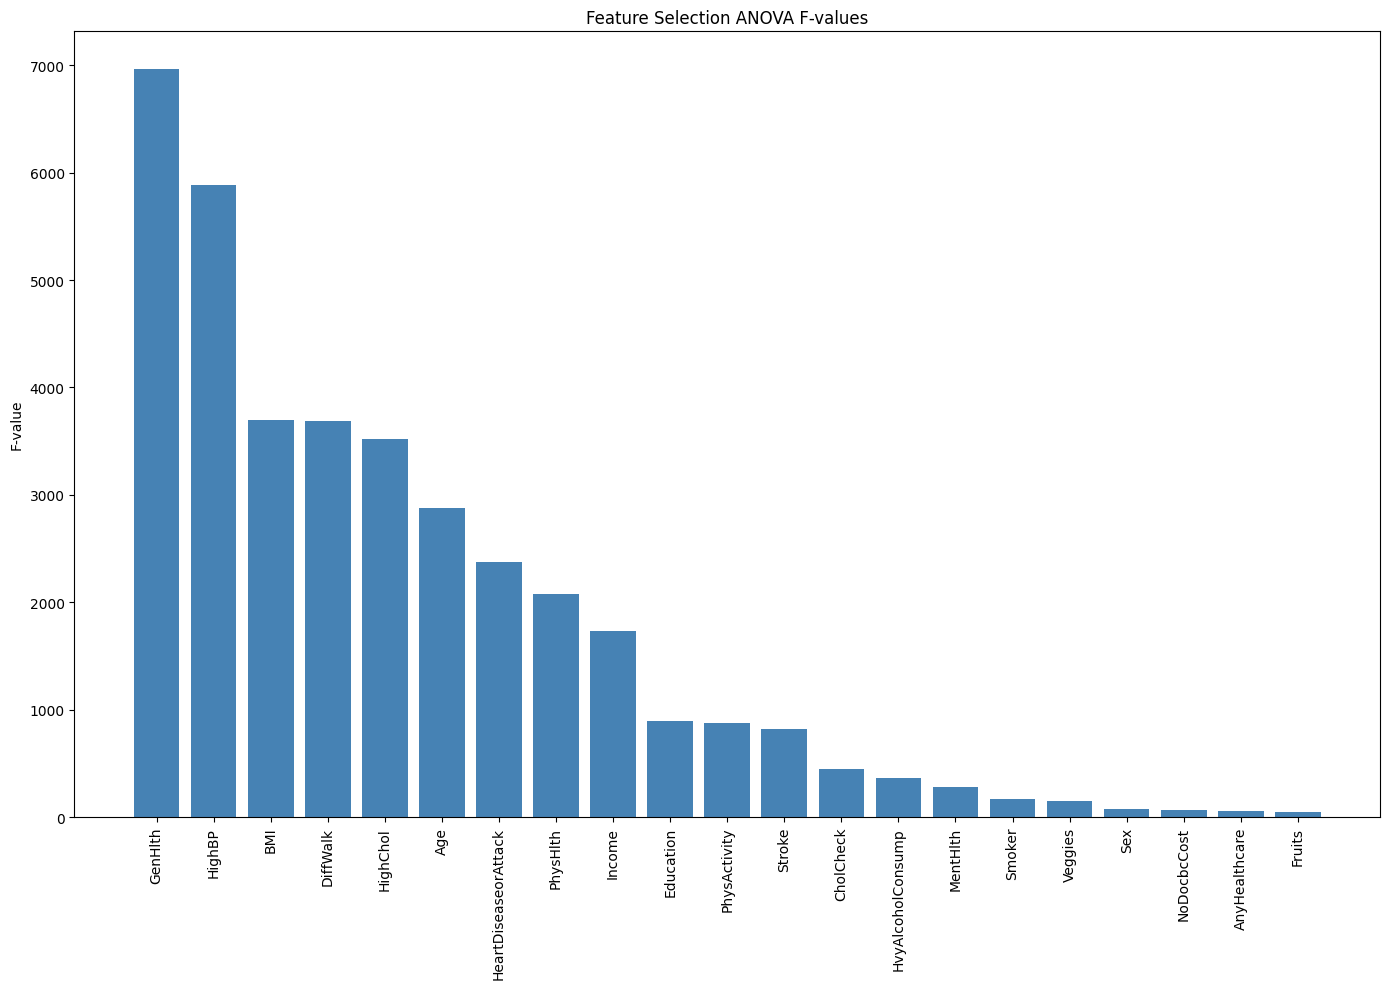
\includegraphics[width=1.15\textwidth]{datapreprocessing/feat-selection.png}
    \caption{Feature Importance Scores from Random Forest Classifier}
\end{figure}

\begin{figure}[H]
    \hspace{-1.5cm}
    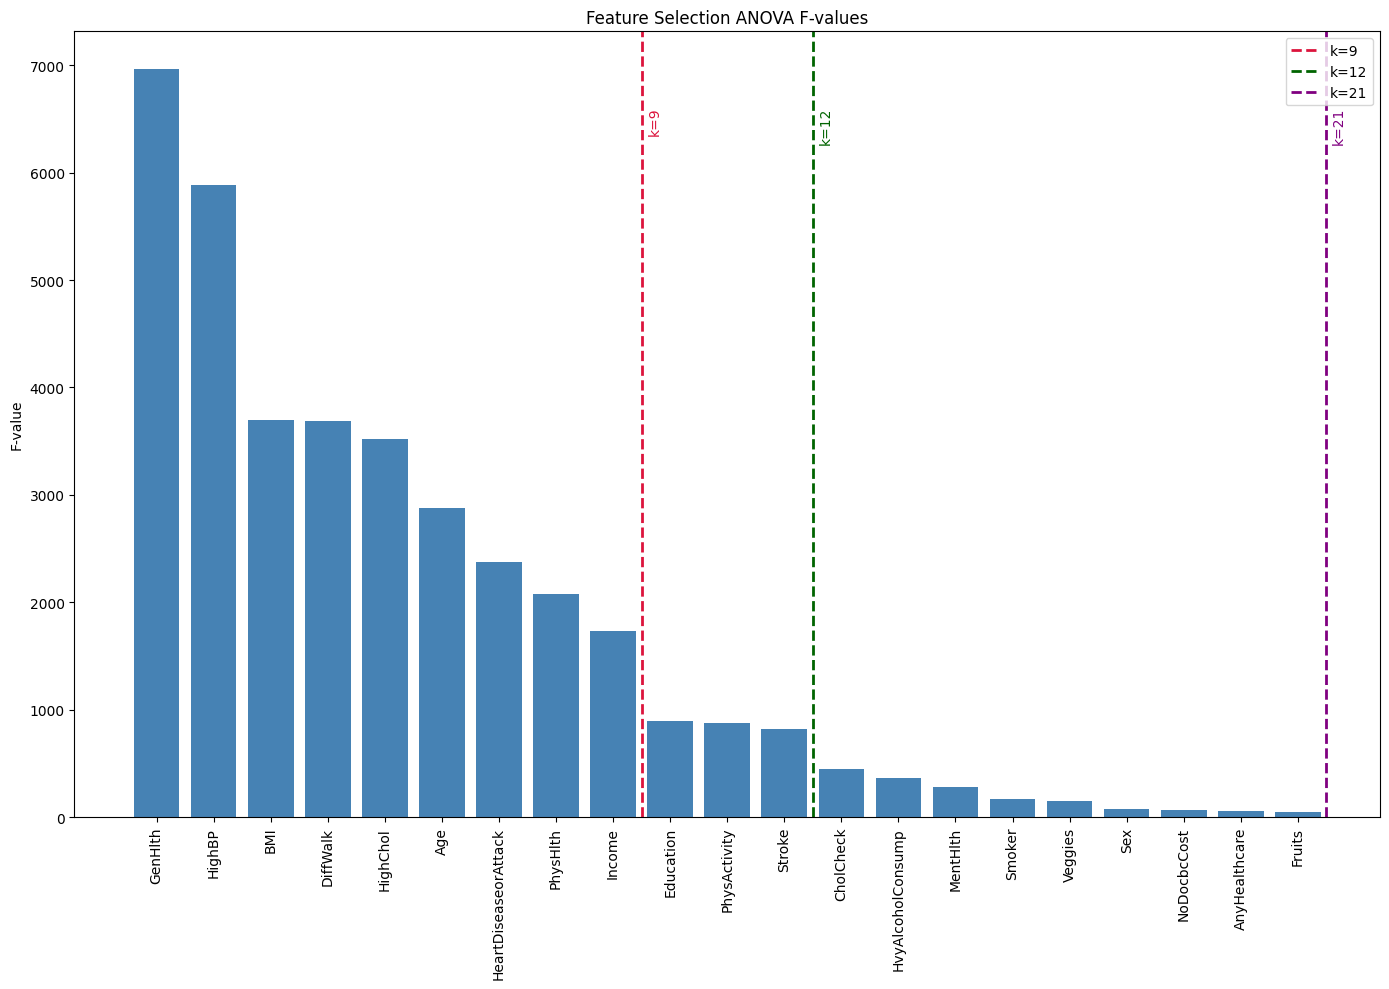
\includegraphics[width=1.15\textwidth]{datapreprocessing/feat-k-selected.png}
    \caption{Features Selected Based on Feature Importance Scores}
\end{figure}

\newpage
\noindent The values of \(k\) were selected using an elbow-point interpretation of the ranked feature-importance curve. The main bend appears around \(k=9\), after which score gains become more gradual. We then added \(k=12\) as a post-elbow sensitivity check and \(k=21\) as a near-plateau reference to measure the effect of keeping a wider feature set.

\vspace{1cm}
\hrule
\vspace{1cm}
\begin{table}[H]
    \centering
    \caption{Rationale for Choosing Feature Subset Sizes}
    \label{tab:k-selection-rationale}
    \begin{tabular}{p{0.12\textwidth} p{0.28\textwidth} p{0.48\textwidth}}
        \toprule
        \textbf{Value of \(k\)} & \textbf{Selection Goal} & \textbf{Why It Was Selected} \\
        \midrule
        \(k=9\) & Elbow point & Chosen as the primary cutoff where the curve changes from steep to flatter growth, capturing the strongest contributors before diminishing returns dominate. \\ \\
        \(k=12\) & Post-elbow check & Adds a small number of features after the elbow to test whether modest extra complexity provides meaningful performance or stability gains over \(k=9\). \\ \\
        \(k=21\) & Near-plateau reference & Represents the Base Dataset after applying the balancing on it. \\
        \bottomrule
    \end{tabular}
\end{table}

\newpage

\section{Data Splitting}
The dataset was split into :
\begin{itemize}
    \item Training Set (70\%)
    \item Validation Set (10\%)
    \item Test Set (20\%)
\end{itemize}
The Use of \texttt{stratify} parameter in the \texttt{train\_test\_split} function ensured that the class distribution is preserved across the training, validation, and test sets.

\vspace{1 cm}
\hrule
\vspace{1 cm}

\section{Data Balancing}
Data balancing was performed in two ways:
\begin{itemize}
    \item SMOTE (Synthetic Minority Over-sampling Technique)
    \item Random Under-sampling
\end{itemize}

\newpage
\subsection{SMOTE}
\begin{figure}[H]
    \hspace{-2.3cm}
    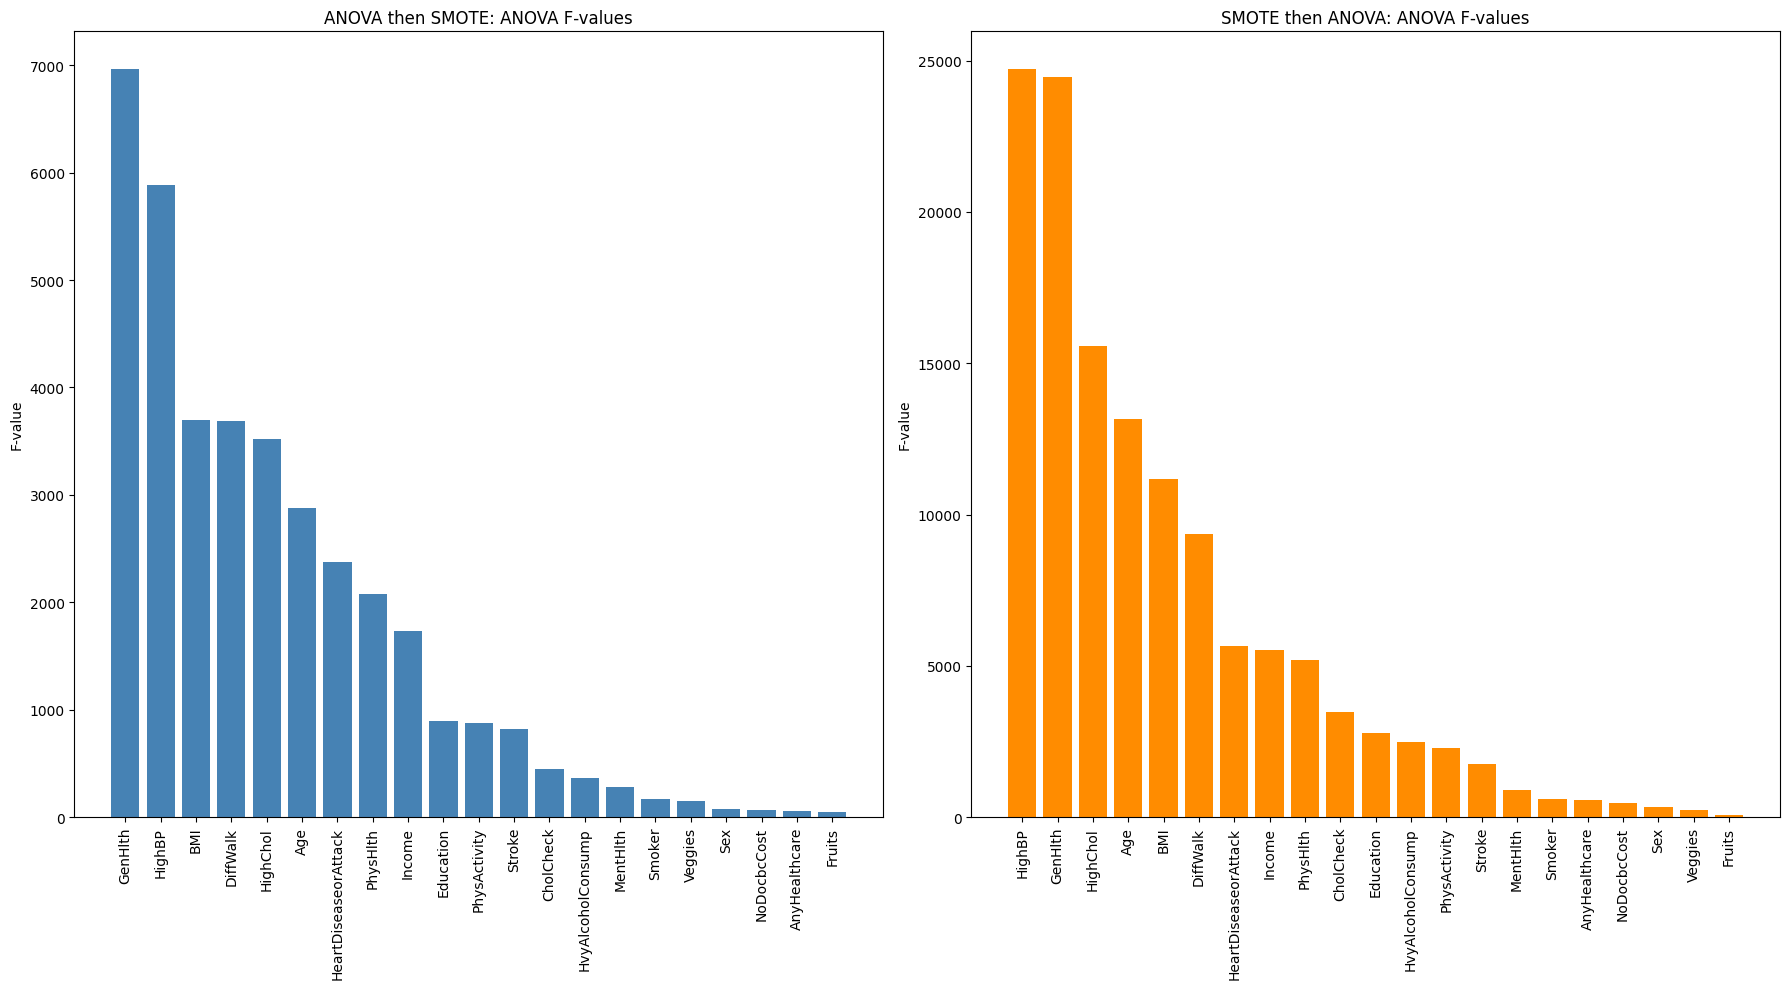
\includegraphics[width=1.3\textwidth,height=1\textwidth,keepaspectratio]{datapreprocessing/smote/correlation.png}
    \caption{Comparison of ANOVA F1-Values before and after balancing}
\end{figure}

\begin{figure}[H]
    \hspace{-2.6cm}
    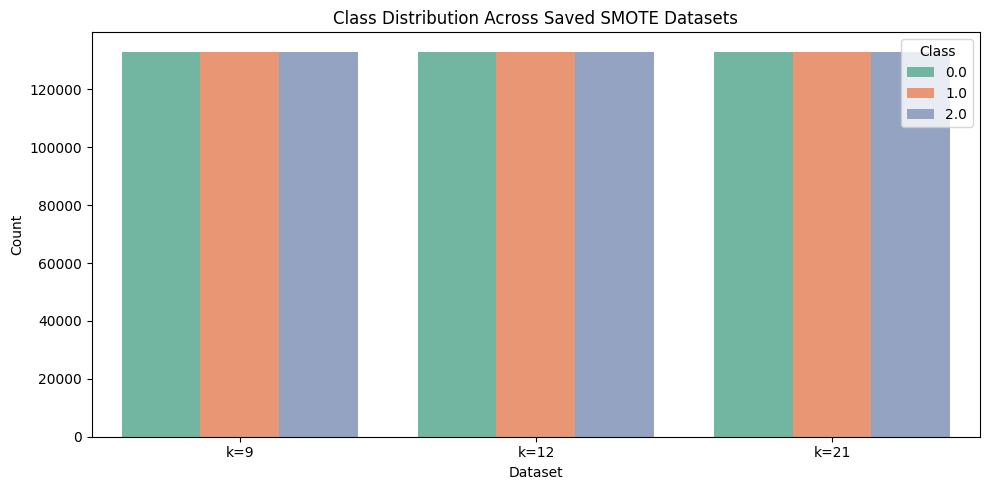
\includegraphics[width=1.3\textwidth,height=1\textwidth,keepaspectratio]{datapreprocessing/smote/class-dist.png}
    \caption{SMOTE Class Distribution}
\end{figure}

\newpage
\begin{figure}[H]
    \hspace{-2.3cm}
    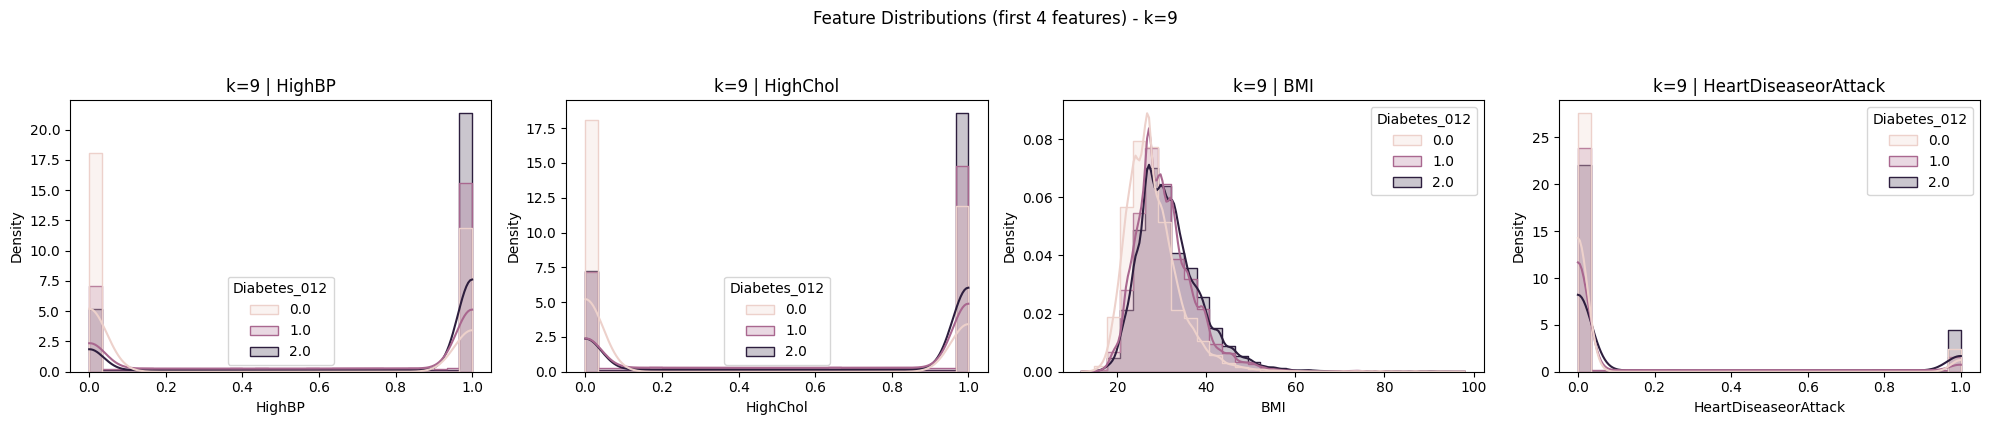
\includegraphics[width=1.3\textwidth,height=1\textwidth,keepaspectratio]{datapreprocessing/smote/f-dist9.png}
    \caption{Feature Distribution for \(k=9\) after SMOTE Balancing}
\end{figure}
\begin{figure}[H]
    \hspace{-2.3cm}
    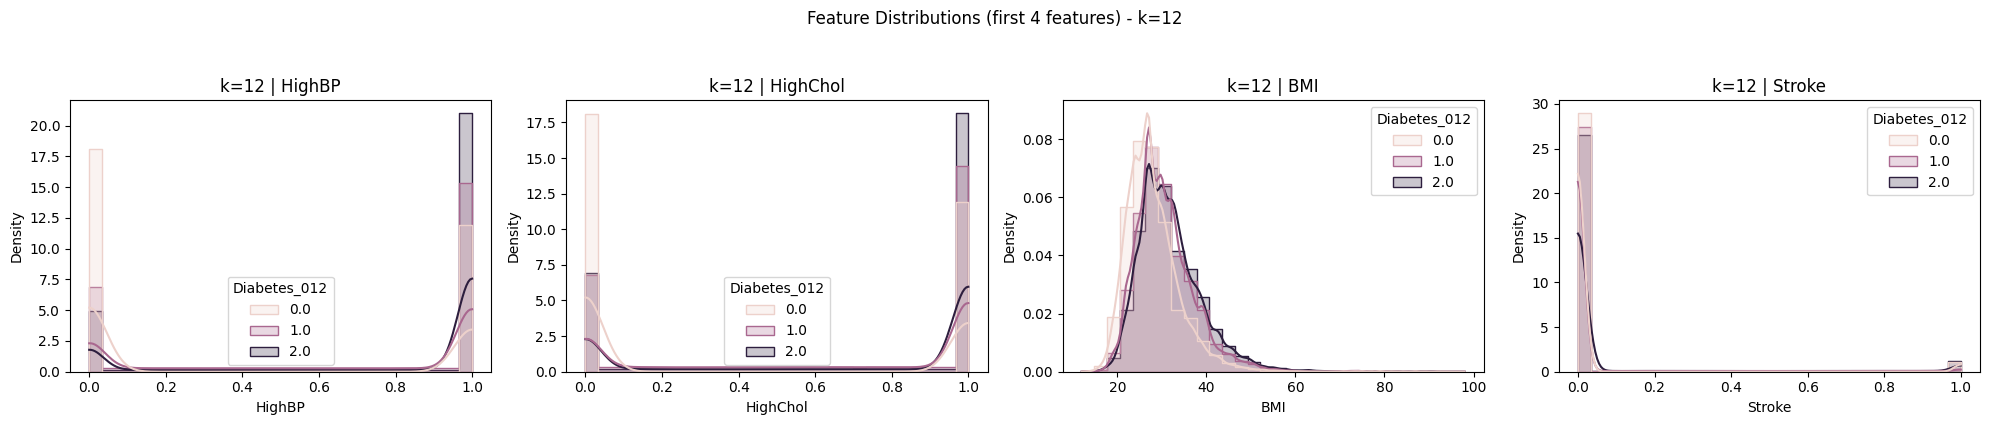
\includegraphics[width=1.3\textwidth,height=1\textwidth,keepaspectratio]{datapreprocessing/smote/f-dist12.png}
    \caption{Feature Distribution for \(k=12\) after SMOTE Balancing}
\end{figure}

\begin{figure}[H]
    \hspace{-2.3cm}
    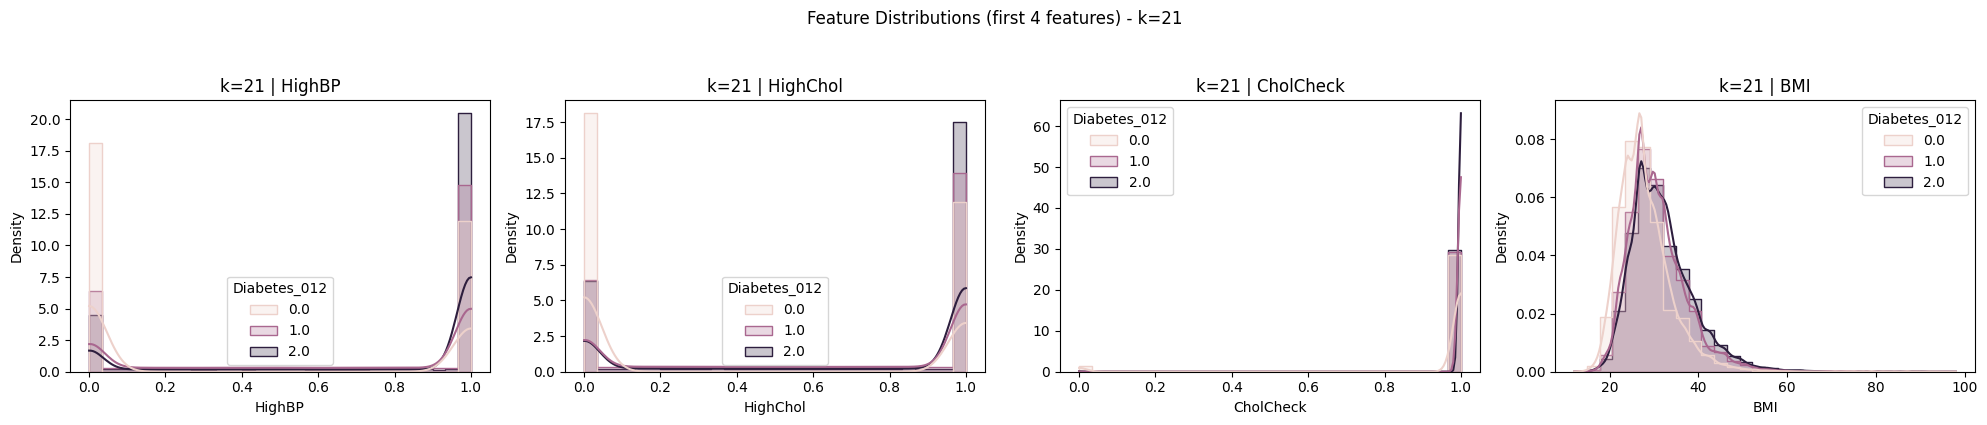
\includegraphics[width=1.3\textwidth,height=1\textwidth,keepaspectratio]{datapreprocessing/smote/f-dist21.png}
    \caption{Feature Distribution for \(k=21\) after SMOTE Balancing}
\end{figure}

\newpage
\subsection{Random Under-sampling}
\begin{figure}[H]
    \hspace{-2.3cm}
    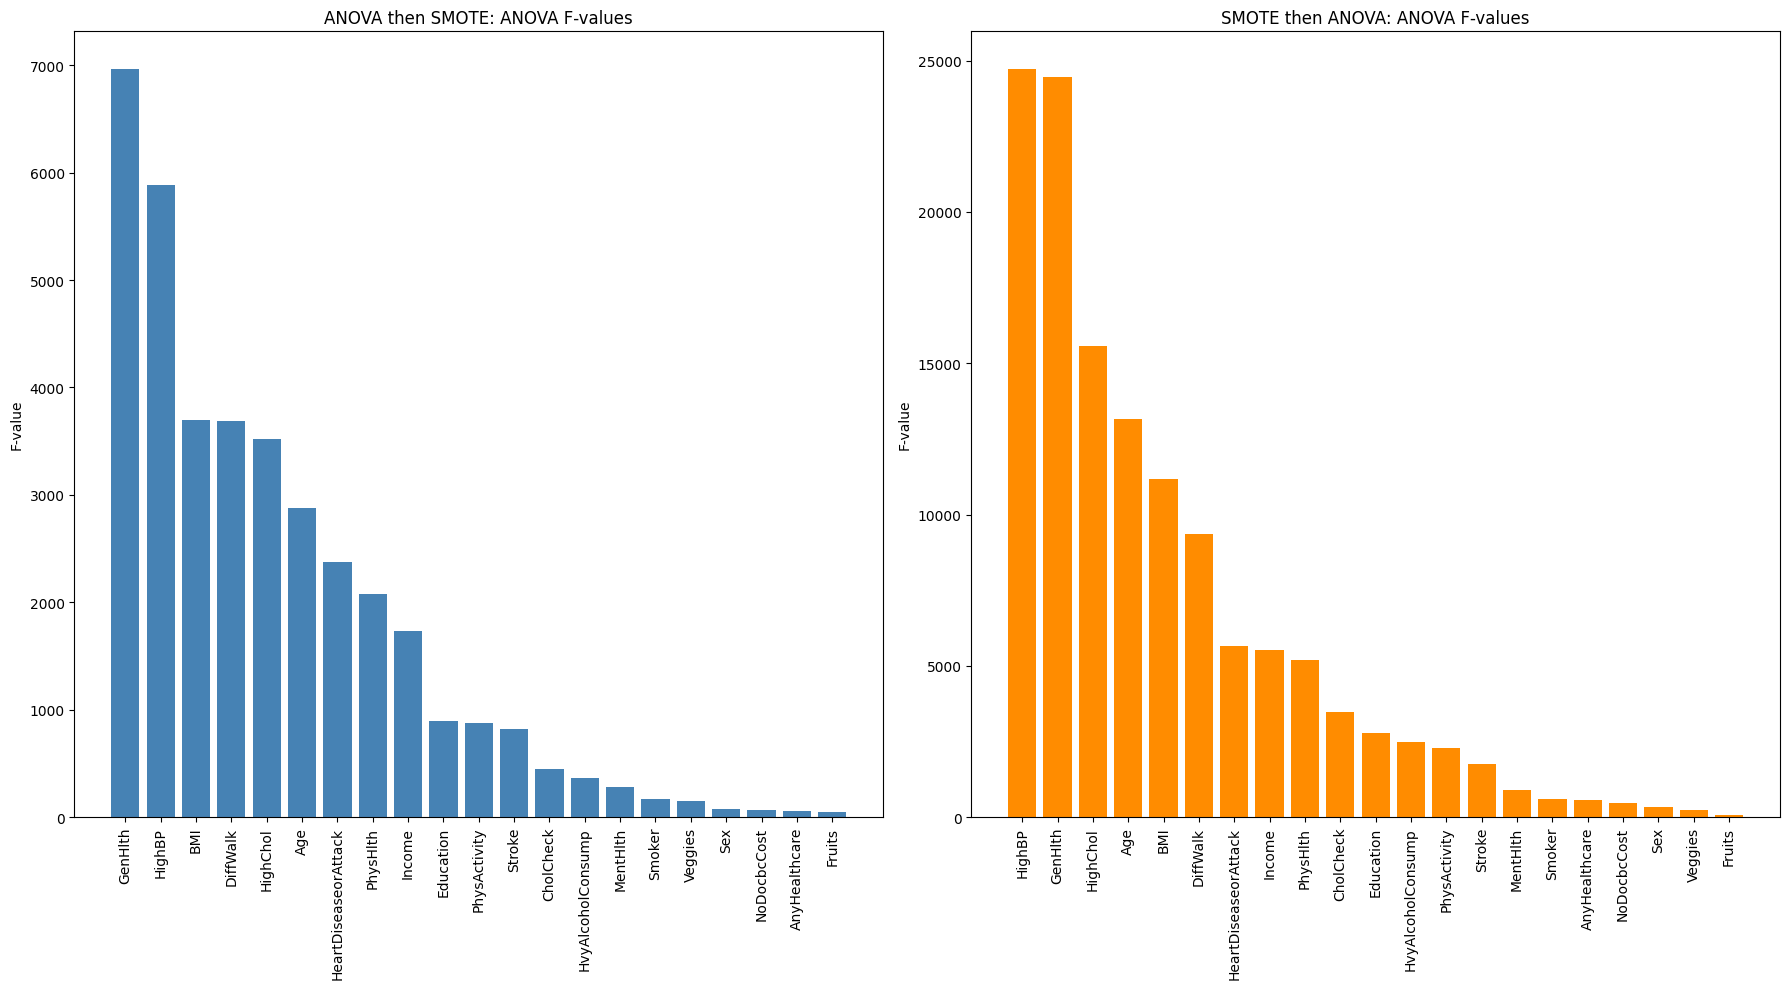
\includegraphics[width=1.3\textwidth,height=1\textwidth,keepaspectratio]{datapreprocessing/smote/correlation.png}
    \caption{Comparison of ANOVA F1-Values before and after balancing}
\end{figure}

\begin{figure}[H]
    \hspace{-2.6cm}
    
\includegraphics[width=1.3\textwidth,height=1\textwidth,keepaspectratio]{datapreprocessing/under-sample/class-dist.png}
    \caption{Random Under-sampling Class Distribution}
\end{figure}

\newpage
\begin{figure}[H]
    \hspace{-2.3cm}
    
\includegraphics[width=1.3\textwidth,height=1\textwidth,keepaspectratio]{datapreprocessing/under-sample/f-dist9.png}
    \caption{Feature Distribution for \(k=9\) after Random Under-sampling}
\end{figure}
\begin{figure}[H]
    \hspace{-2.3cm}
    
\includegraphics[width=1.3\textwidth,height=1\textwidth,keepaspectratio]{datapreprocessing/under-sample/f-dist12.png}
    \caption{Feature Distribution for \(k=12\) after Random Under-sampling}
\end{figure}

\begin{figure}[H]
    \hspace{-2.3cm}
    
\includegraphics[width=1.3\textwidth,height=1\textwidth,keepaspectratio]{datapreprocessing/under-sample/f-dist21.png}
    \caption{Feature Distribution for \(k=21\) after Random Under-sampling}
\end{figure}

\newpage
\chapter{K-Nearest Neighbors (KNN)}
\section{Overview}
In this chapter, we will discuss the training of the K-Nearest Neighbors (KNN) algorithm for diabetes risk prediction. We will cover the following topics:
\begin{itemize}
    \item Evaluation Metrics
    \item Confusion Matrix
\end{itemize}

\section{Evaluation Metrics}
\begin{table}[H]
    \centering
    \caption{KNN Performance Metrics Across Dataset Variants}
    \label{tab:knn-metrics-summary}
    \small
    \begin{tabular}{lcccc}
        \toprule
        \textbf{Model Variant} & \textbf{Accuracy} & \textbf{F1 Micro} & \textbf{F1 Macro} & \textbf{F1 Weighted} \\
        \midrule
        Baseline & 0.8219 & 0.8219 & 0.4016 & 0.7993 \\
        Oversampling ($k=9$) & 0.7298 & 0.7298 & 0.4276 & 0.7579 \\
        Oversampling ($k=12$) & 0.7302 & 0.7302 & 0.4315 & 0.7592 \\
        Undersampling ($k=9$) & 0.5870 & 0.5870 & 0.4020 & 0.6714 \\
        Undersampling ($k=12$) & 0.5908 & 0.5908 & 0.4017 & 0.6735 \\
        \bottomrule
    \end{tabular}
\end{table}

\section{Confusion Matrix}
\begin{figure}[H]
    \hspace{-2.3cm}
    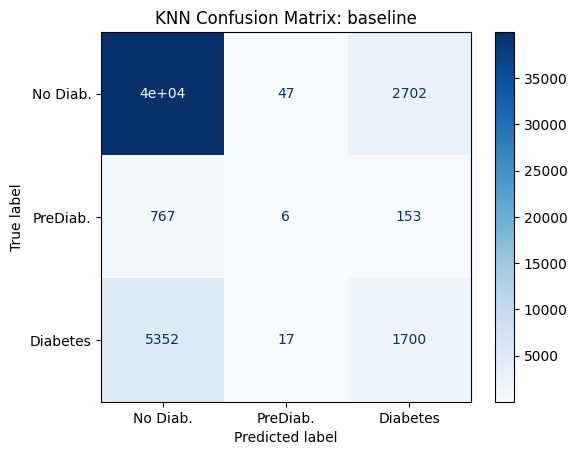
\includegraphics[width=1.3\textwidth,height=1\textwidth,keepaspectratio]{models/knn/base.png}
    \caption{Baseline KNN Confusion Matrix}
\end{figure}

\begin{figure}[H]
    \hspace{-2.3cm}
    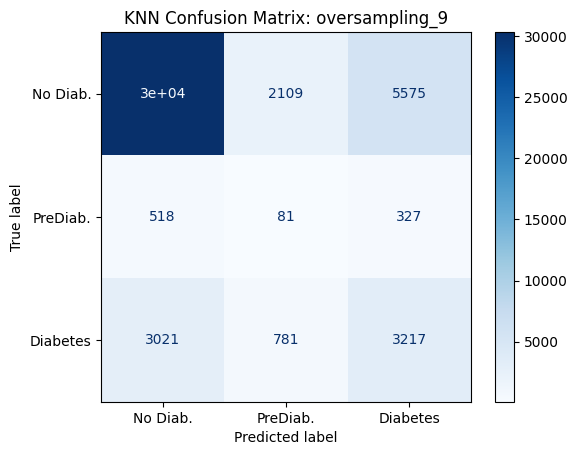
\includegraphics[width=1.3\textwidth,height=1\textwidth,keepaspectratio]{models/knn/smote9.png}
    \caption{SMOTE K=9 KNN Confusion Matrix}
\end{figure}

\begin{figure}[H]
    \hspace{-2.3cm}
    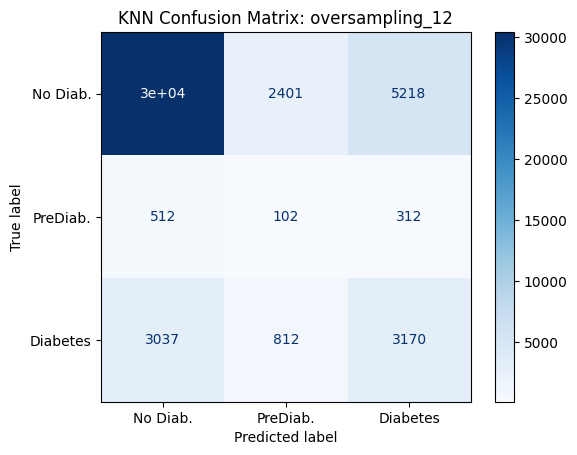
\includegraphics[width=1.3\textwidth,height=1\textwidth,keepaspectratio]{models/knn/smote12.png}
    \caption{SMOTE K=12 KNN Confusion Matrix}
\end{figure}


\begin{figure}[H]
    \hspace{-2.3cm}
    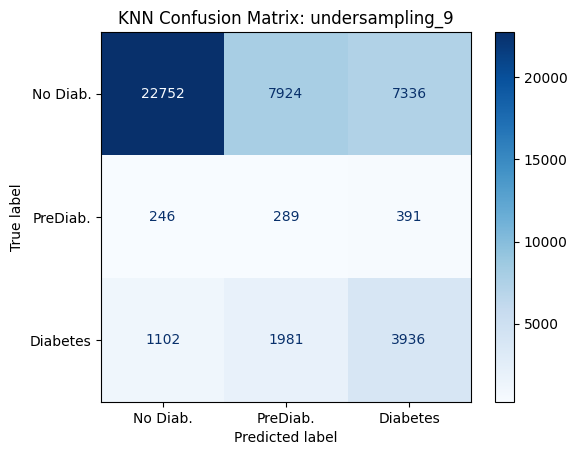
\includegraphics[width=1.3\textwidth,height=1\textwidth,keepaspectratio]{models/knn/under9.png}
    \caption{Random Under-sampling K=9 KNN Confusion Matrix}
\end{figure}

\begin{figure}[H]
    \hspace{-2.3cm}
    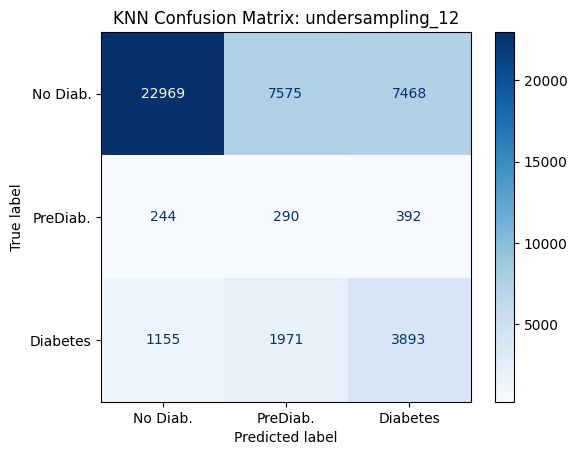
\includegraphics[width=1.3\textwidth,height=1\textwidth,keepaspectratio]{models/knn/under12.png}
    \caption{Random Under-sampling K=12 KNN Confusion Matrix}
\end{figure}


\newpage
\chapter{Softmax}
\section{Overview}
In this chapter, we will discuss the training of the Softmax Regression algorithm for diabetes risk prediction.
\section{Evaluation Metrics}

\begin{table}[H]
    \centering
    \caption{Softmax Performance Metrics Across Dataset Variants}
    \label{tab:softmax-metrics-summary}
    \scriptsize
    \resizebox{\textwidth}{!}{%
    \begin{tabular}{llccccccc}
        \toprule
        \textbf{Dataset} & \textbf{Backend} & \textbf{Best C} & \textbf{Test Accuracy} & \textbf{Recall Macro} & \textbf{Recall Weighted} & \textbf{F1 Micro} & \textbf{F1 Macro} & \textbf{F1 Weighted} \\
        \midrule
        Baseline & gpu & 10.00 & 0.833540 & 0.387032 & 0.833540 & 0.833540 & 0.395527 & 0.793064 \\
        Oversampling ($k=9$) & gpu & 0.01 & 0.630633 & 0.510483 & 0.630633 & 0.630633 & 0.424164 & 0.703156 \\
        Undersampling ($k=9$) & gpu & 3.00 & 0.628022 & 0.510808 & 0.628022 & 0.628022 & 0.423739 & 0.701904 \\
        Undersampling ($k=12$) & gpu & 10.00 & 0.626325 & 0.507914 & 0.626325 & 0.626325 & 0.422190 & 0.700986 \\
        Oversampling ($k=12$) & gpu & 0.01 & 0.628870 & 0.505213 & 0.628870 & 0.628870 & 0.422111 & 0.701823 \\
        Undersampling ($k=21$) & gpu & 0.01 & 0.624366 & 0.511308 & 0.624366 & 0.624366 & 0.421937 & 0.699614 \\
        Oversampling ($k=21$) & gpu & 0.01 & 0.624976 & 0.510879 & 0.624976 & 0.624976 & 0.421735 & 0.699790 \\
        \bottomrule
    \end{tabular}%
    }
\end{table}

\section{Confusion Matrix}
\begin{figure}[H]
    \hspace{-2.3cm}
    
\includegraphics[width=1.3\textwidth,height=1\textwidth,keepaspectratio]{models/soft/base.png}
    \caption{Baseline Softmax Confusion Matrix}
\end{figure}

\begin{figure}[H]
    \hspace{-2.3cm}
    
\includegraphics[width=1.3\textwidth,height=1\textwidth,keepaspectratio]{models/soft/smote9.png}
    \caption{SMOTE K=9 Softmax Confusion Matrix}
\end{figure}

\begin{figure}[H]
    \hspace{-2.3cm}
    
\includegraphics[width=1.3\textwidth,height=1\textwidth,keepaspectratio]{models/soft/smote12.png}
    \caption{SMOTE K=12 Softmax Confusion Matrix}
\end{figure}

\begin{figure}[H]
    \hspace{-2.3cm}
    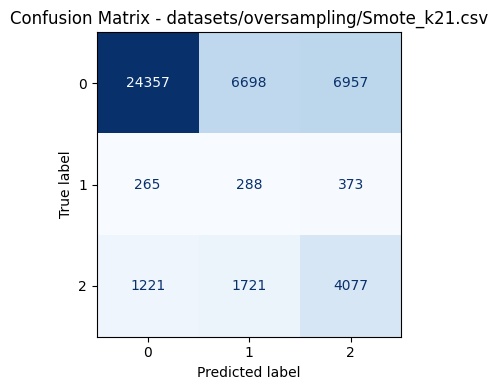
\includegraphics[width=1.3\textwidth,height=1\textwidth,keepaspectratio]{models/soft/smote21.png}
    \caption{SMOTE K=12 Softmax Confusion Matrix}
\end{figure}


\begin{figure}[H]
    \hspace{-2.3cm}
    
\includegraphics[width=1.3\textwidth,height=1\textwidth,keepaspectratio]{models/soft/under9.png}
    \caption{Random Under-sampling K=9 Softmax Confusion Matrix}
\end{figure}

\begin{figure}[H]
    \hspace{-2.3cm}
    
\includegraphics[width=1.3\textwidth,height=1\textwidth,keepaspectratio]{models/soft/under12.png}
    \caption{Random Under-sampling K=12 Softmax Confusion Matrix}
\end{figure}

\begin{figure}[H]
    \hspace{-2.3cm}
    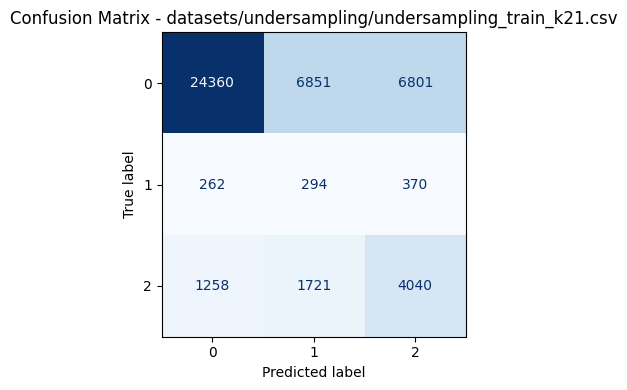
\includegraphics[width=1.3\textwidth,height=1\textwidth,keepaspectratio]{models/soft/under21.png}
    \caption{Random Under-sampling K=21 Softmax Confusion Matrix}
\end{figure}


\newpage
\chapter{Neural Networks}
\section{Overview}
In this chapter, we will discuss the training of the Neural Networks for diabetes risk prediction.
\section{Evaluation Metrics}

\begin{table}[H]
    \centering
    \caption{Neural Network Performance Metrics Across Dataset Variants}
    \label{tab:nn-metrics-summary}
    \scriptsize
    \resizebox{\textwidth}{!}{%
    \begin{tabular}{lcccccc}
        \toprule
        \textbf{Model} & \textbf{Accuracy} & \textbf{F1 Micro} & \textbf{F1 Macro} & \textbf{F1 Weighted} & \textbf{Precision (W)} & \textbf{Recall (W)} \\
        \midrule
        base & 0.8493 & 0.8493 & 0.3898 & 0.8077 & 0.8049 & 0.8493 \\
        smote\_k9 & 0.7702 & 0.7702 & 0.4407 & 0.7818 & 0.8068 & 0.7702 \\
        smote\_k12 & 0.7819 & 0.7819 & 0.4468 & 0.7892 & 0.7977 & 0.7819 \\
        smote\_k21 & 0.8298 & 0.8298 & 0.4163 & 0.7999 & 0.7882 & 0.8298 \\
        undersample\_k9 & 0.7048 & 0.7048 & 0.4353 & 0.7431 & 0.8199 & 0.7048 \\
        undersample\_k12 & 0.6216 & 0.6216 & 0.4173 & 0.6929 & 0.8352 & 0.6216 \\
        undersample\_k21 & 0.6423 & 0.6423 & 0.4326 & 0.7162 & 0.8369 & 0.6423 \\
        \bottomrule
    \end{tabular}%
    }
\end{table}

The Neural Network results show a clear trade-off between overall accuracy and minority-class balance. The baseline model achieves the highest \textbf{Accuracy} and \textbf{F1 Micro}, which indicates strong performance on the dominant classes, while SMOTE-based variants improve \textbf{F1 Macro}, suggesting better class-wise balance across all categories. In particular, \texttt{smote\_k12} provides the strongest macro-level performance among the SMOTE settings, whereas under-sampling configurations generally reduce global performance despite relatively competitive weighted precision and recall values. These findings indicate that data-balancing strategy has a direct impact on whether the model prioritizes aggregate correctness or more equitable multi-class behavior.


\section{Confusion Matrix}
\begin{figure}[H]
    \hspace{2.3cm}
    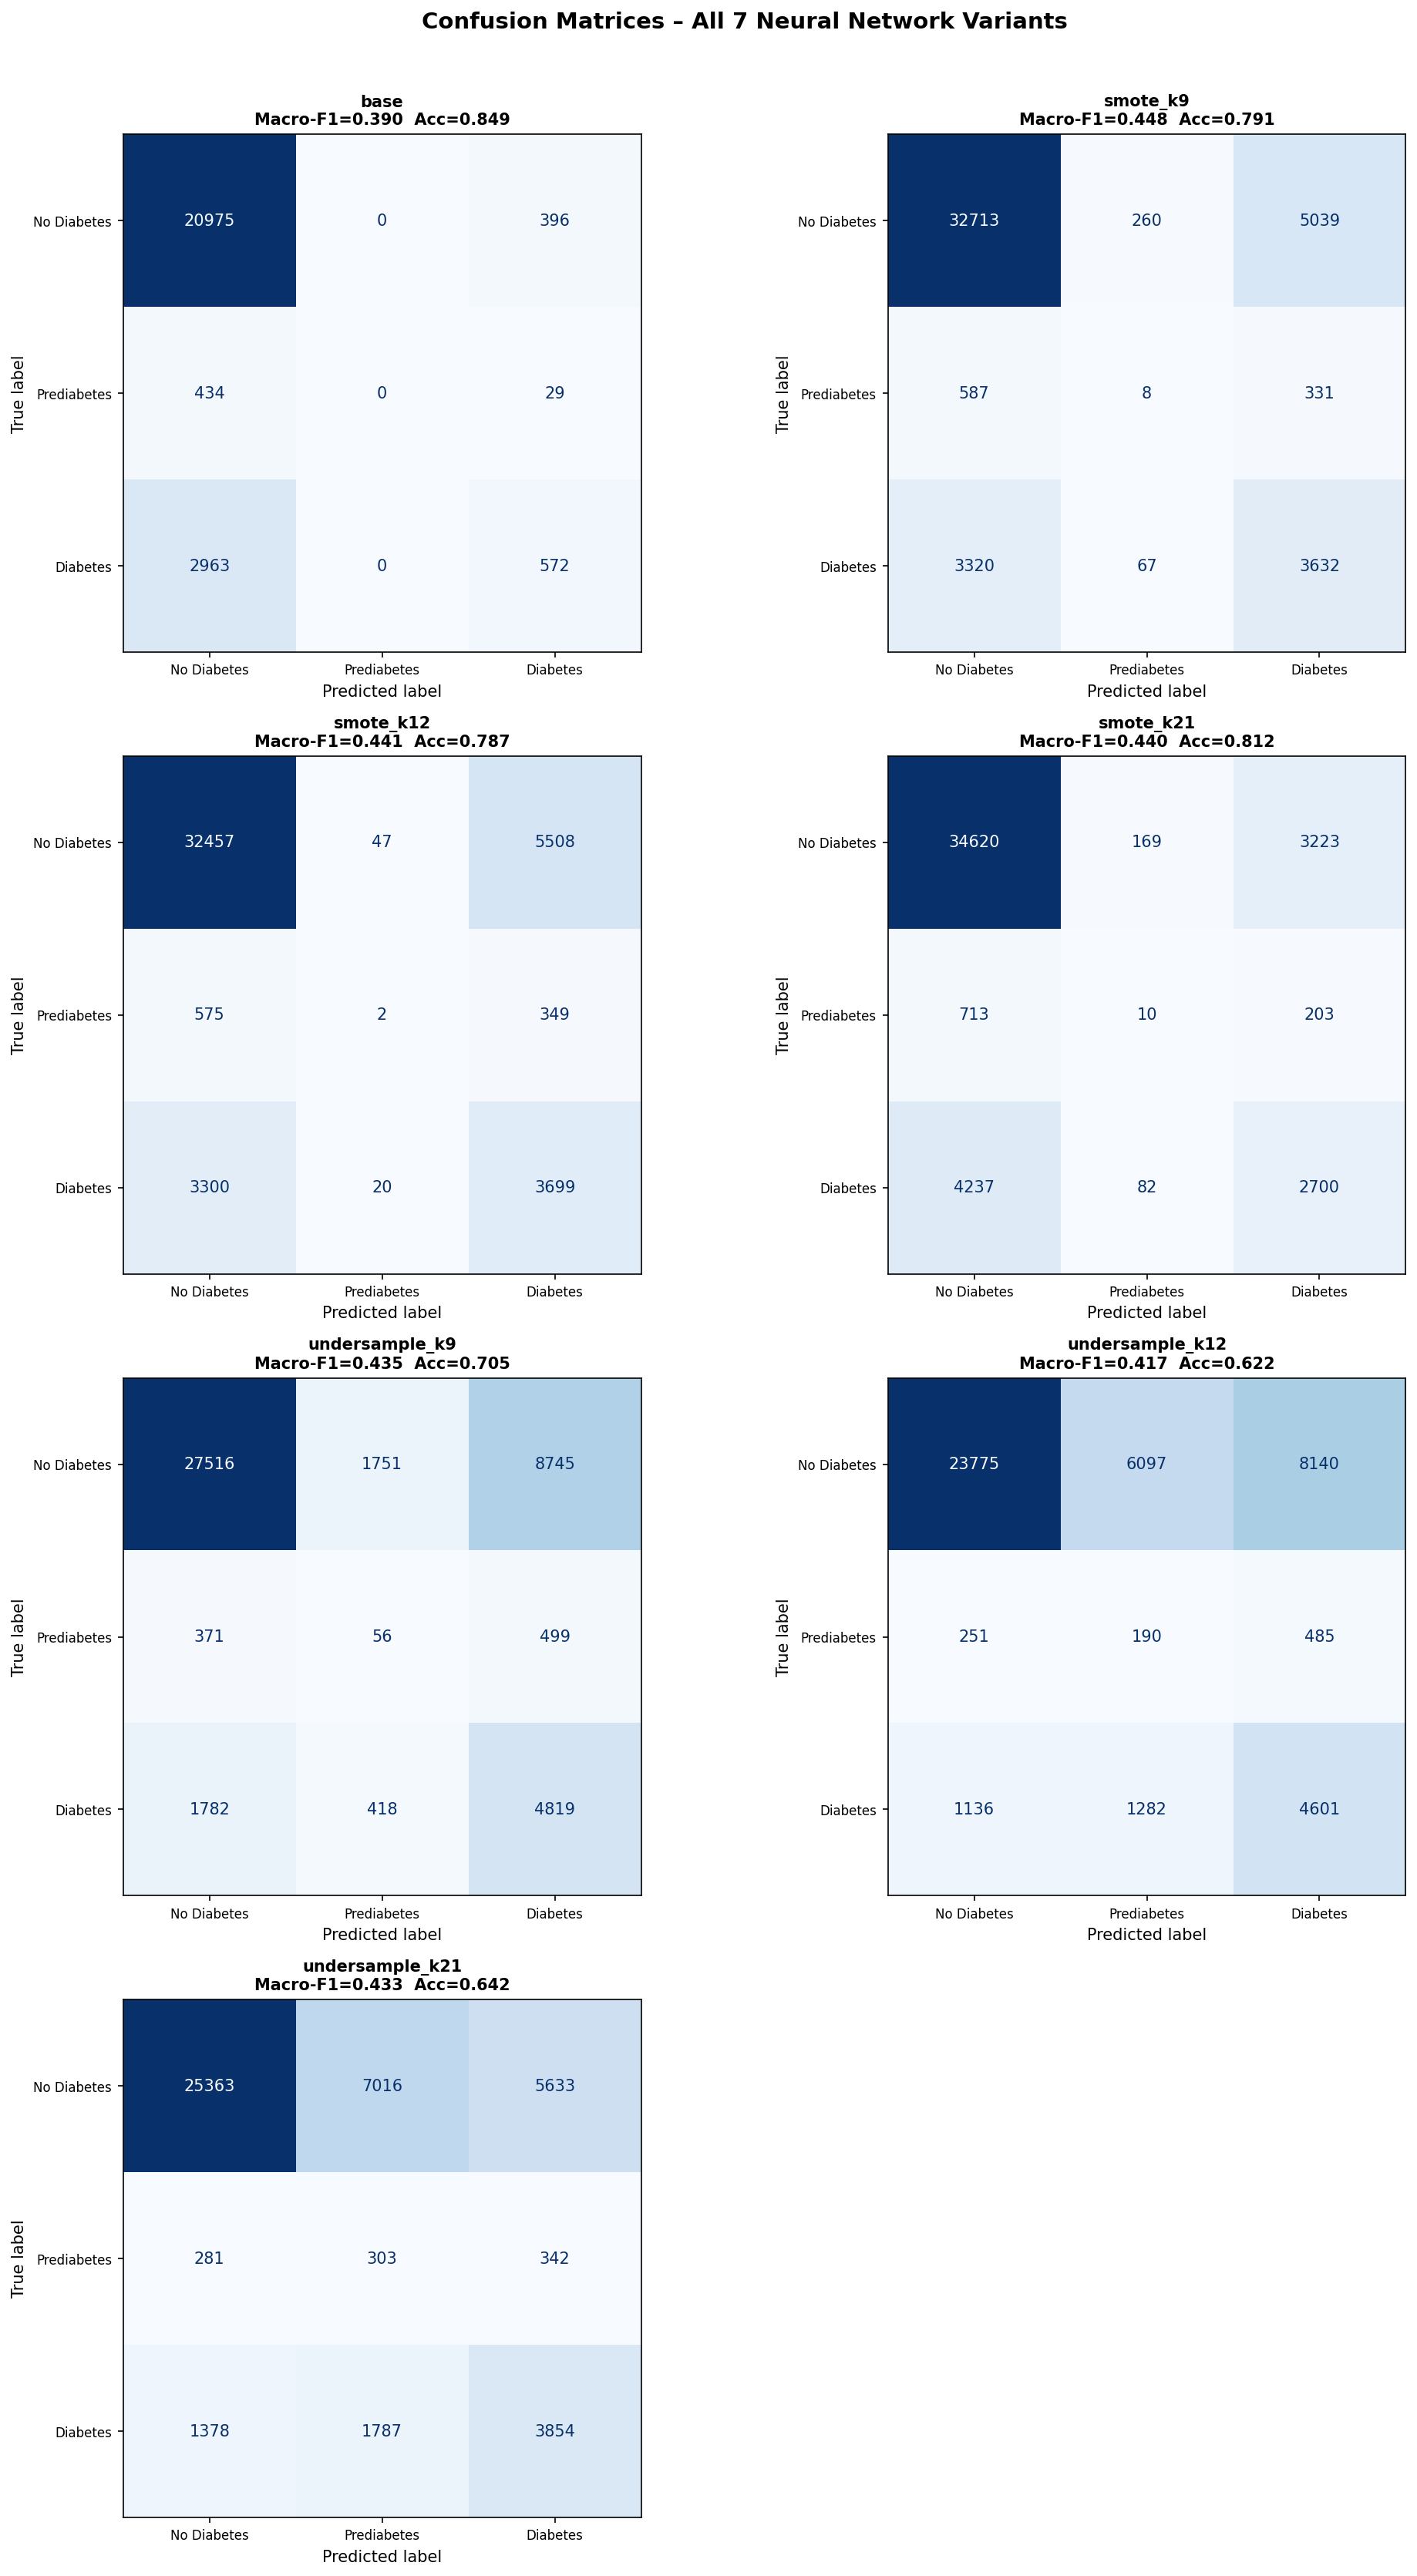
\includegraphics[width=1.5\textwidth,height=1.3\textwidth,keepaspectratio]{nn/confusion_matrices_all_models.png}
    \caption{Baseline Neural Network Confusion Matrix}
\end{figure}


\begin{figure}[H]
    \hspace{2.3cm}
    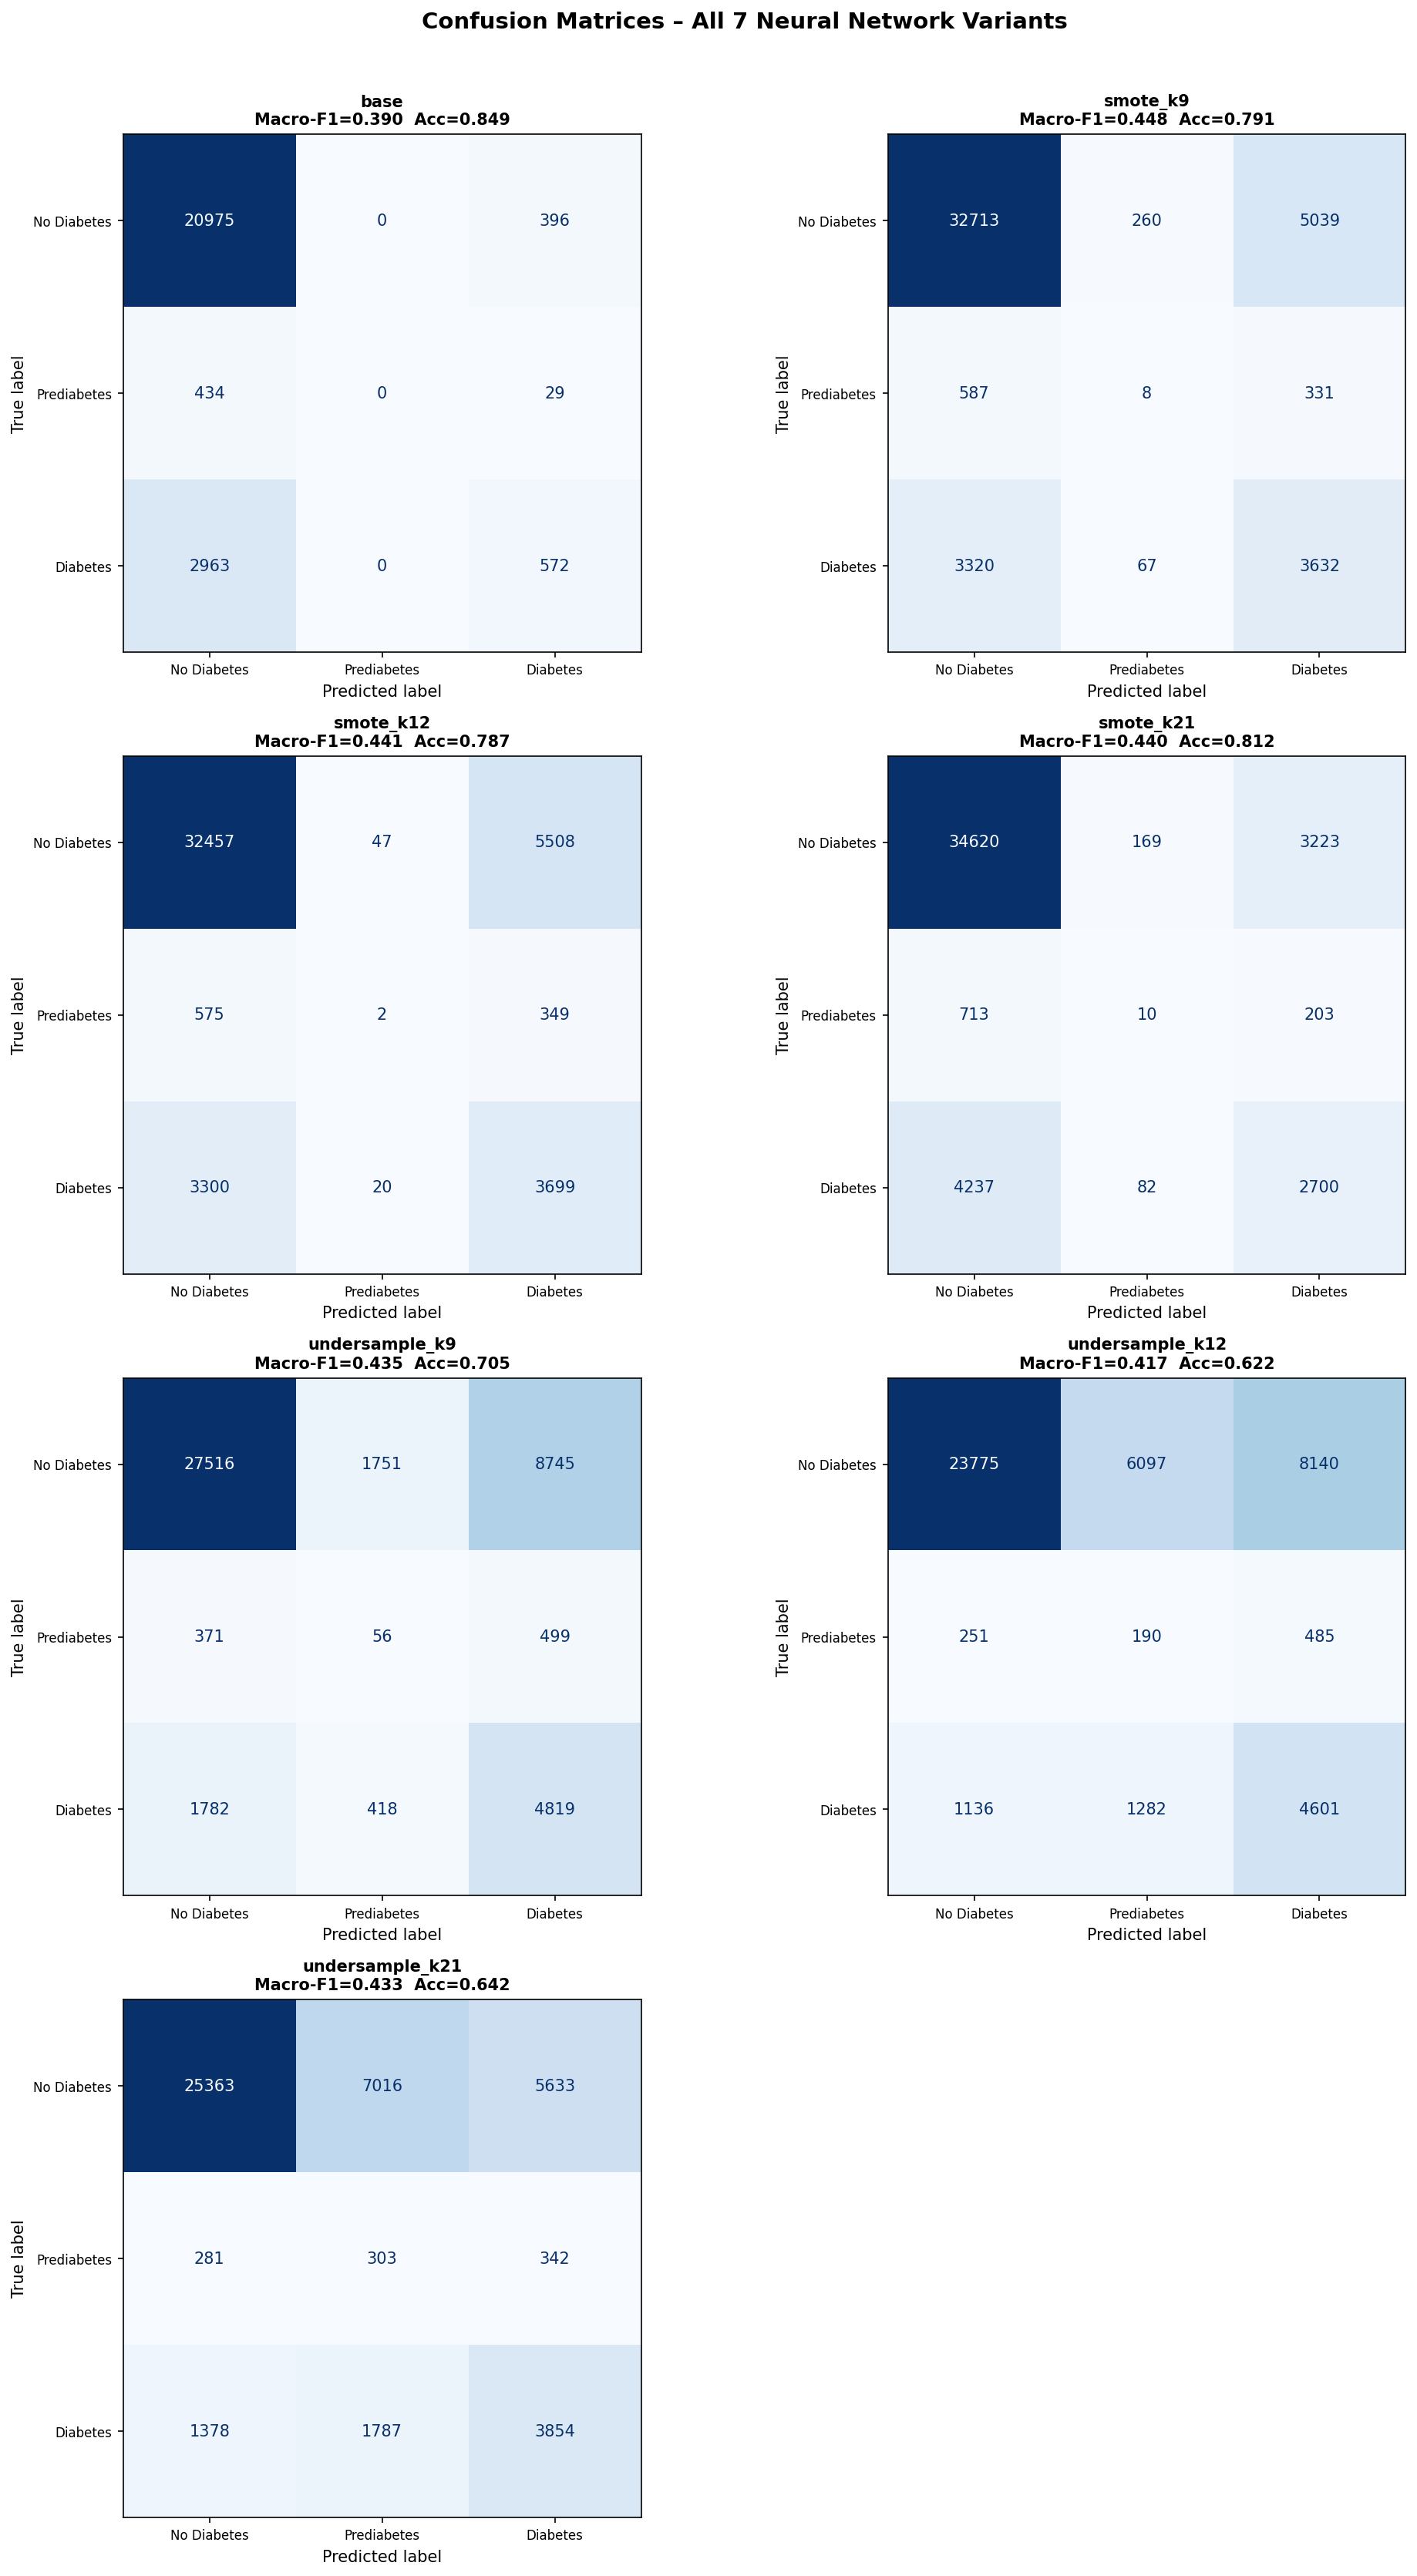
\includegraphics[width=1.5\textwidth,height=1.3\textwidth,keepaspectratio]{nn/confusion_matrices_all_models.png}
    \caption{Confusion Matrices for All Neural Network Models}
\end{figure}

\begin{figure}[H]
    \hspace{-1.3cm}
    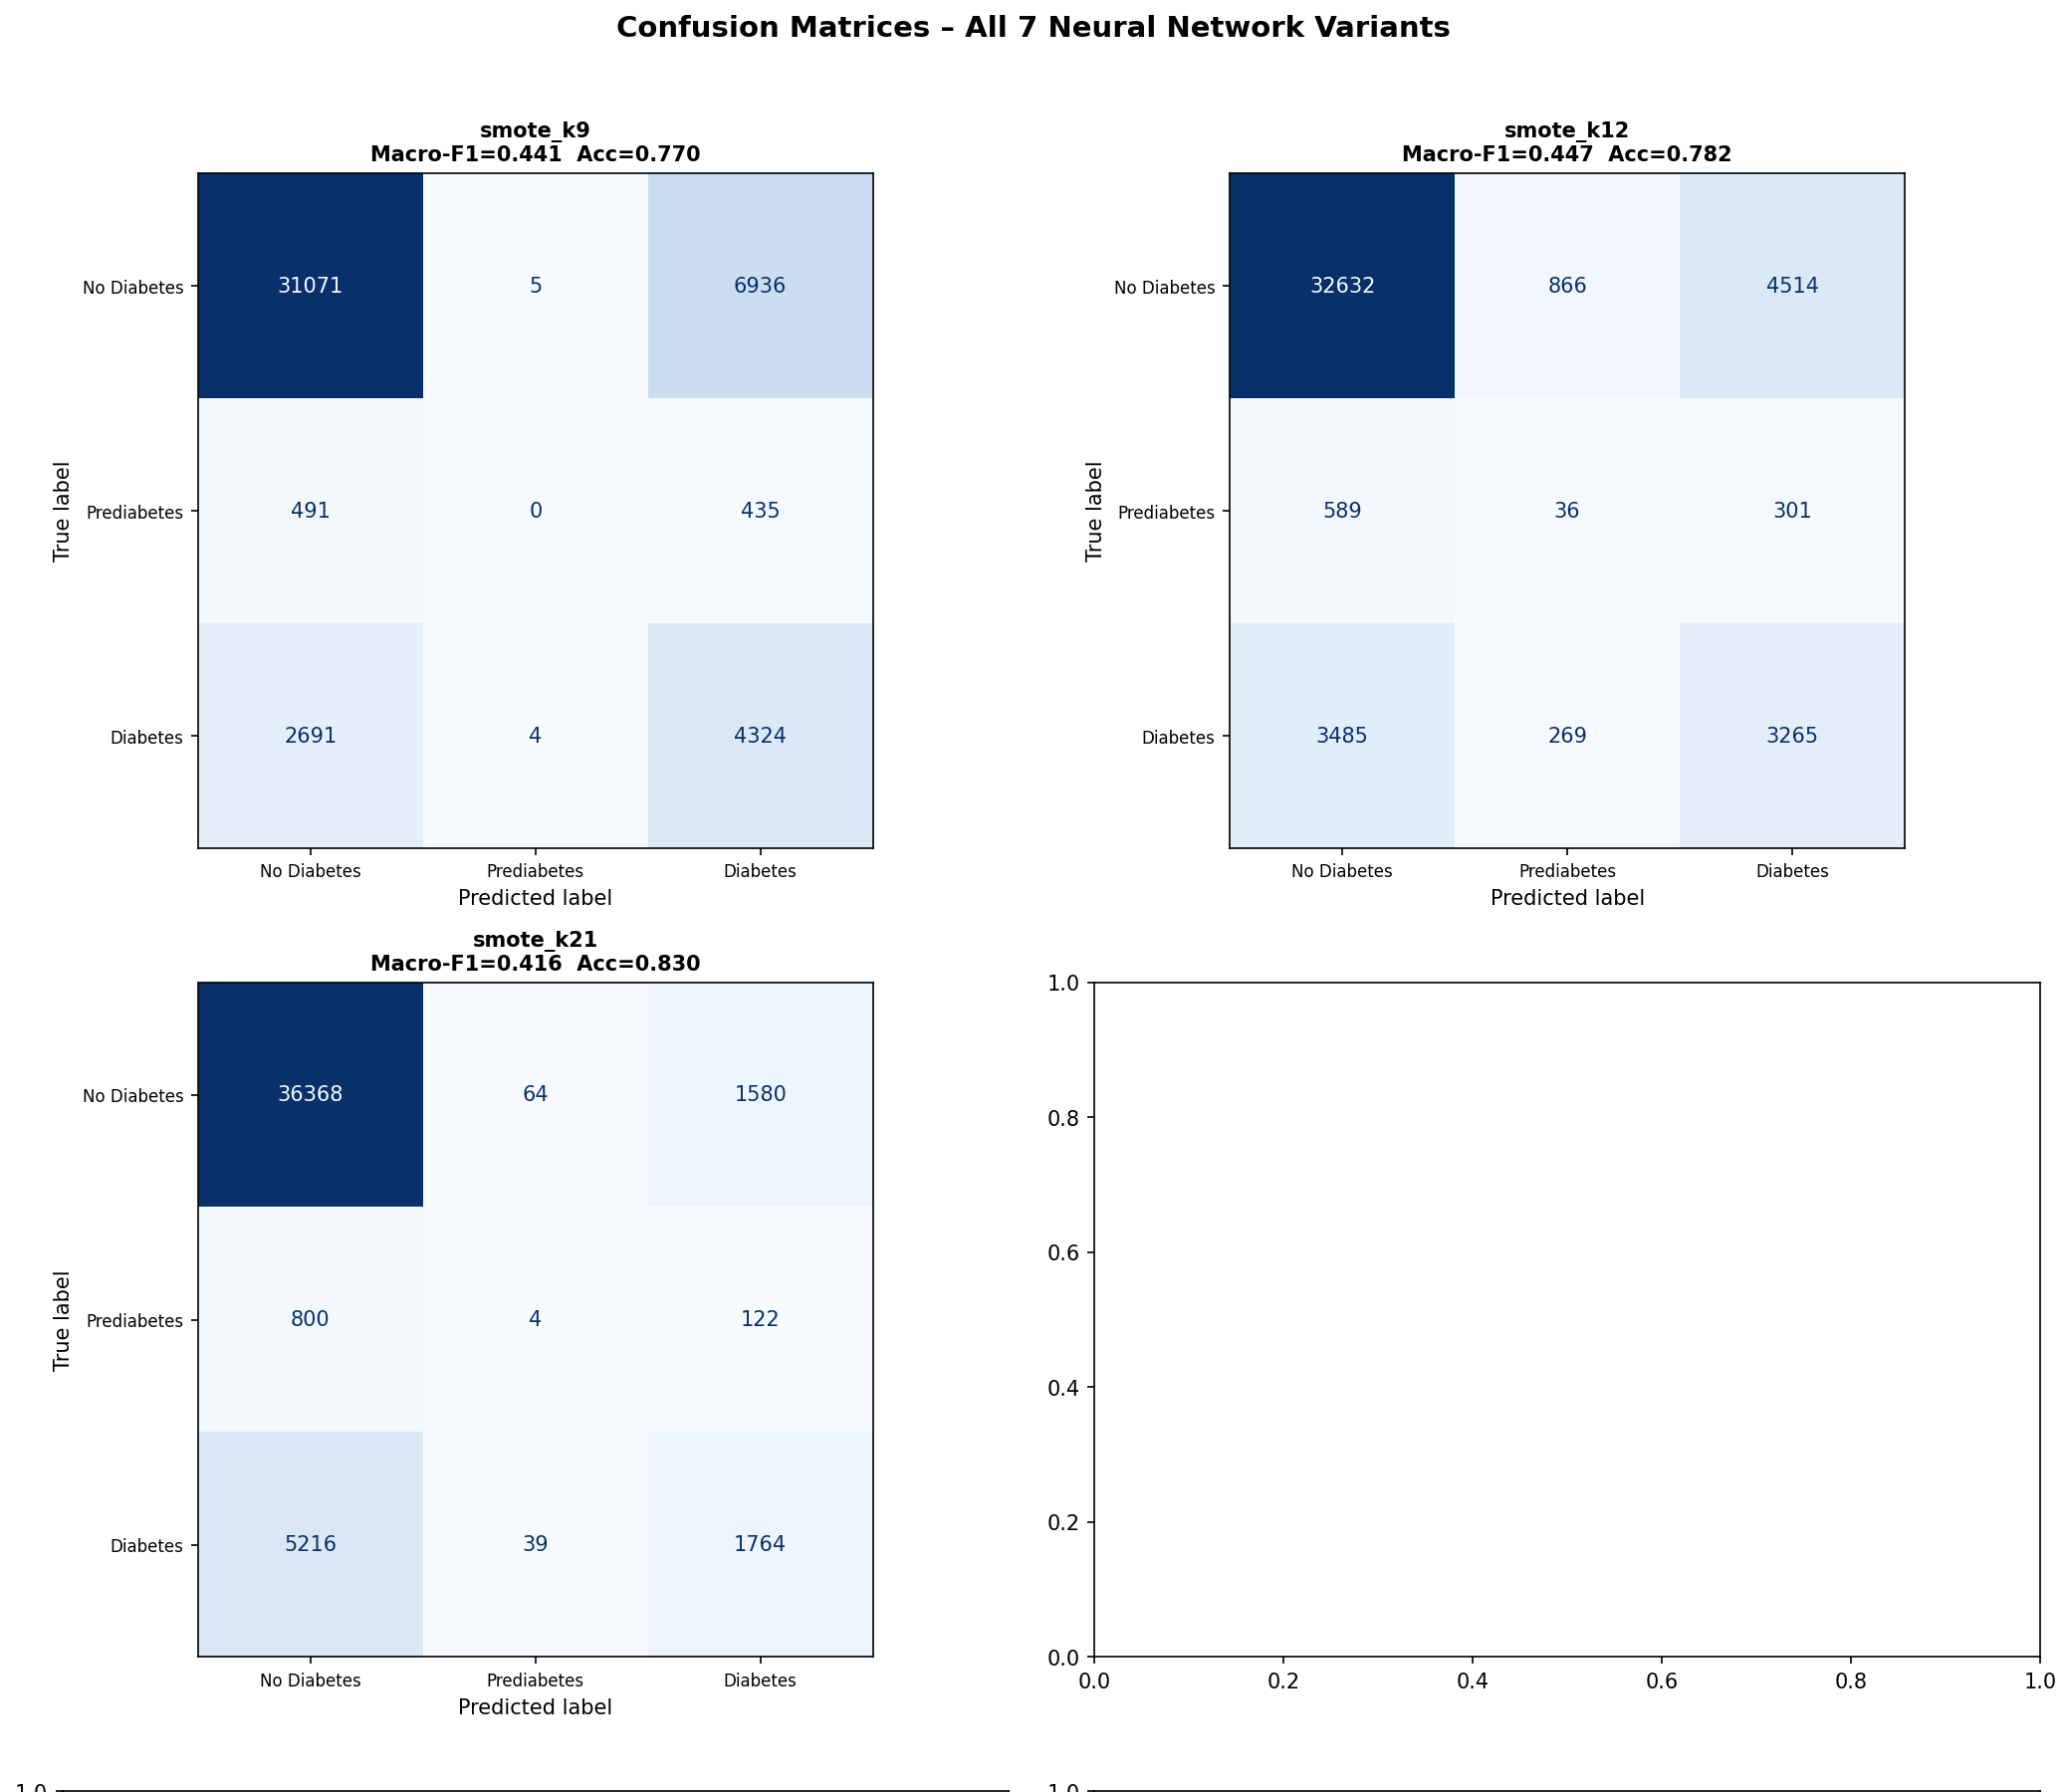
\includegraphics[width=1.1\textwidth,height=1.1\textwidth,keepaspectratio]{nn/confusion_smote.png}
    \caption{Confusion Matrices for All SMOTE Neural Network Models}
\end{figure}

\begin{figure}[H]
    \hspace{-1.3cm}
    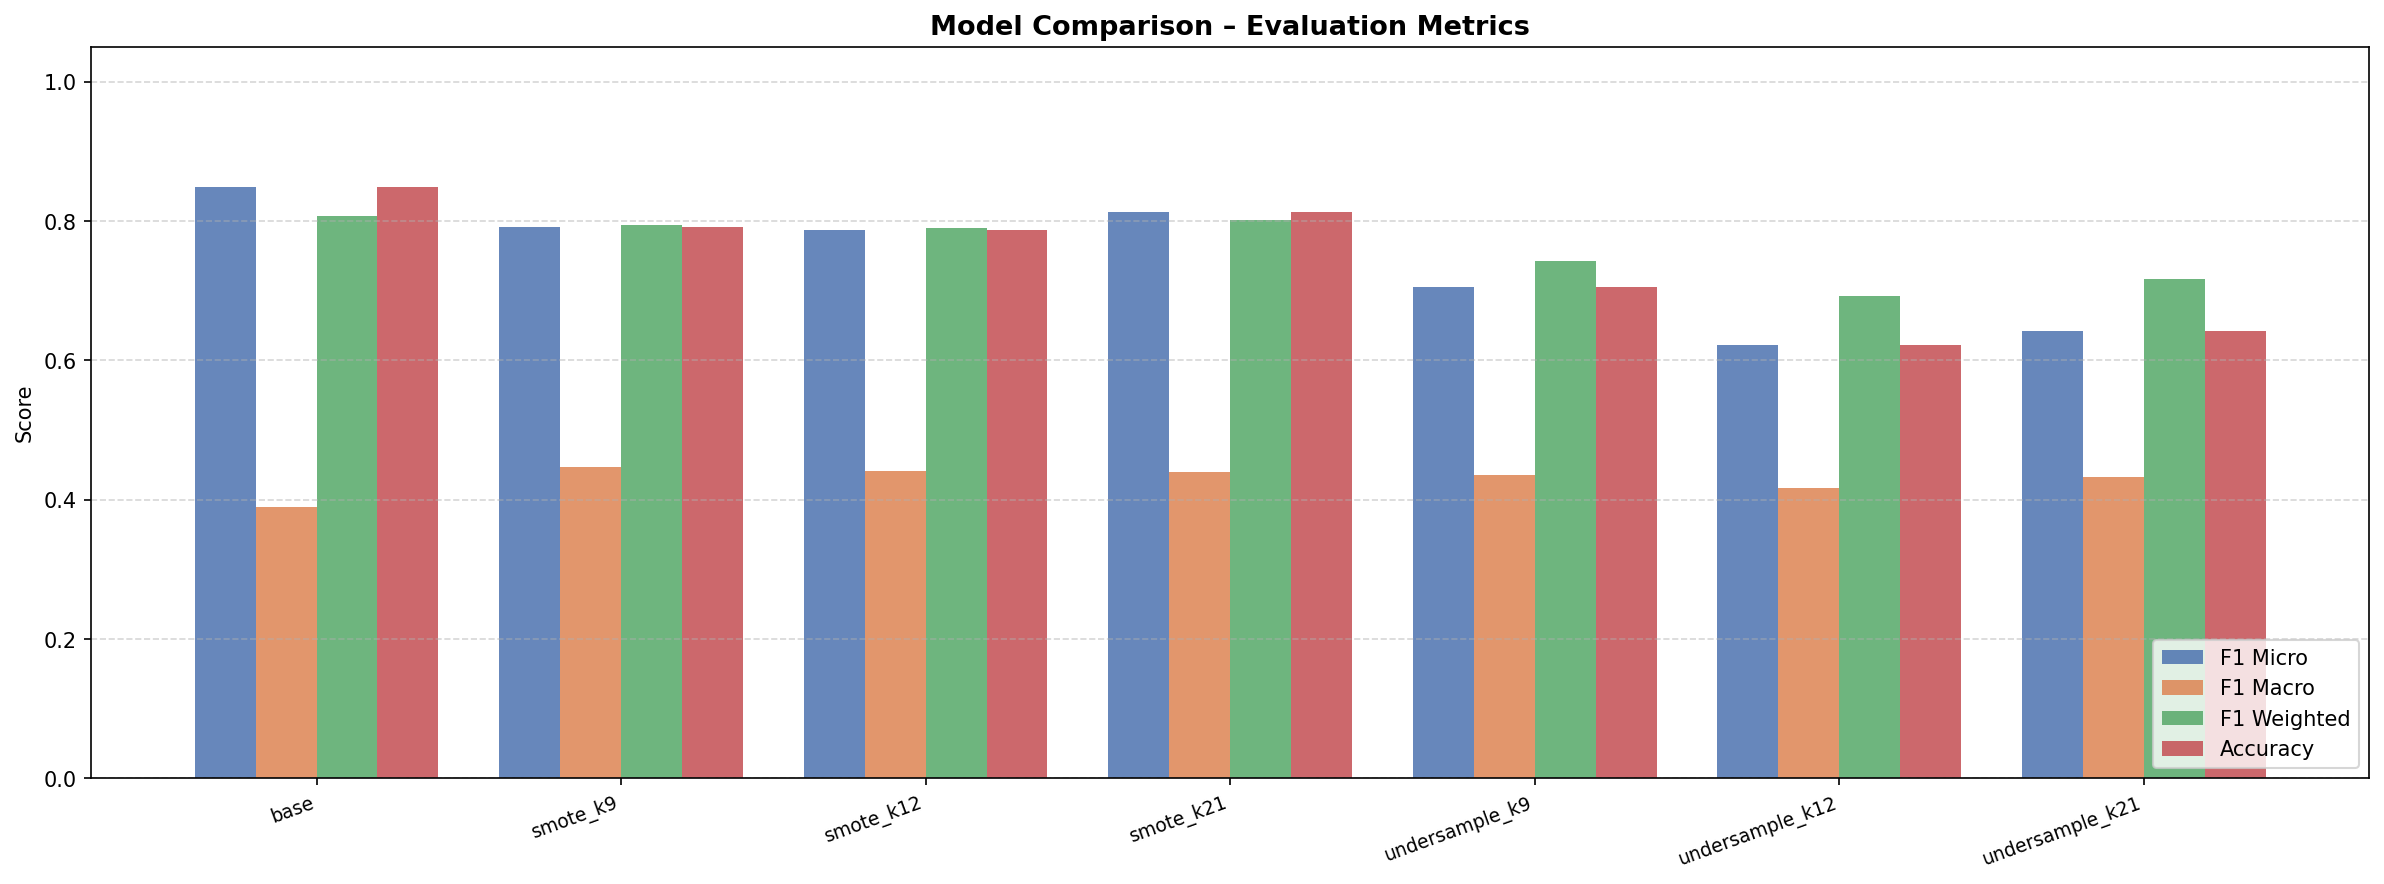
\includegraphics[width=1.1\textwidth,height=1.1\textwidth,keepaspectratio]{nn/metrics_comparison_bar.png}
    \caption{Metrics Comparison for All Neural Network Models}
\end{figure}

\begin{figure}[H]
    \hspace{-1.3cm}
    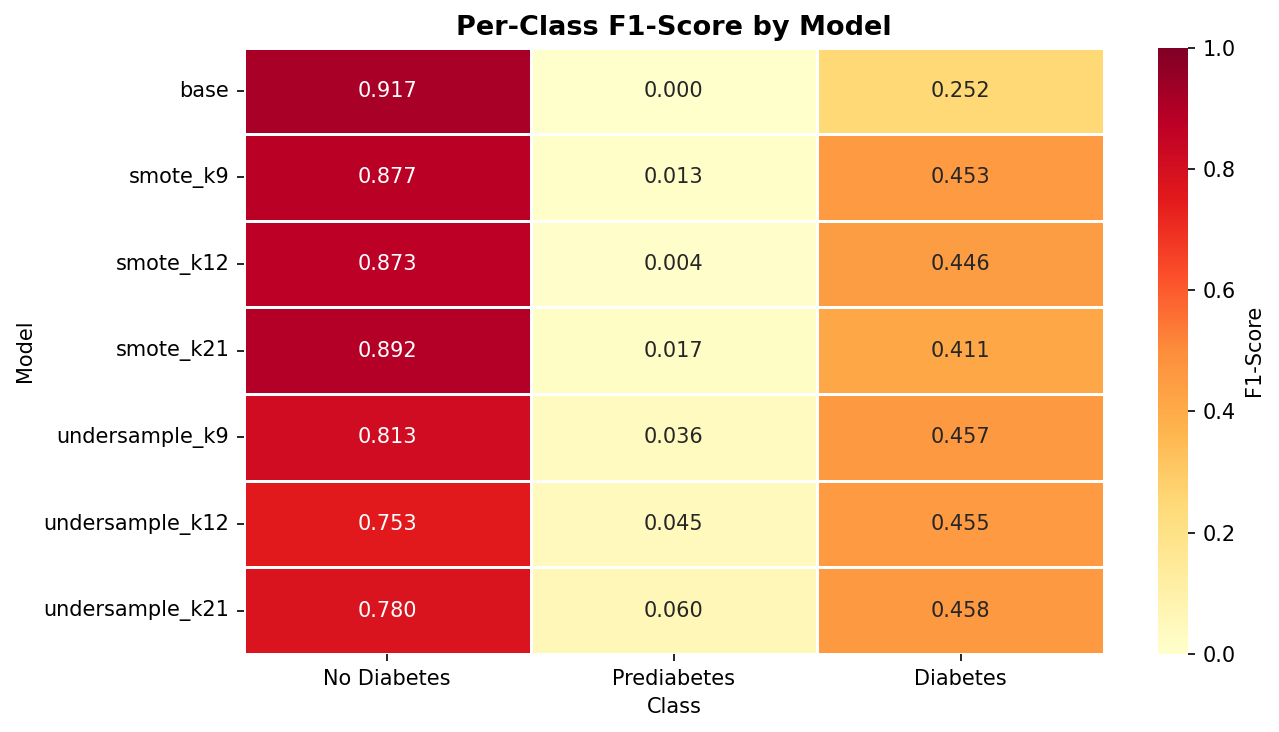
\includegraphics[width=1.1\textwidth,height=1.1\textwidth,keepaspectratio]{nn/per_class_f1_heatmap.png}
    \caption{Per-Class F1-Score Heatmap for Neural Network Models}
\end{figure}


\newpage
\section{TensorBoard Visualizations}
\begin{figure}[H]
    \hspace{-0.3cm}
    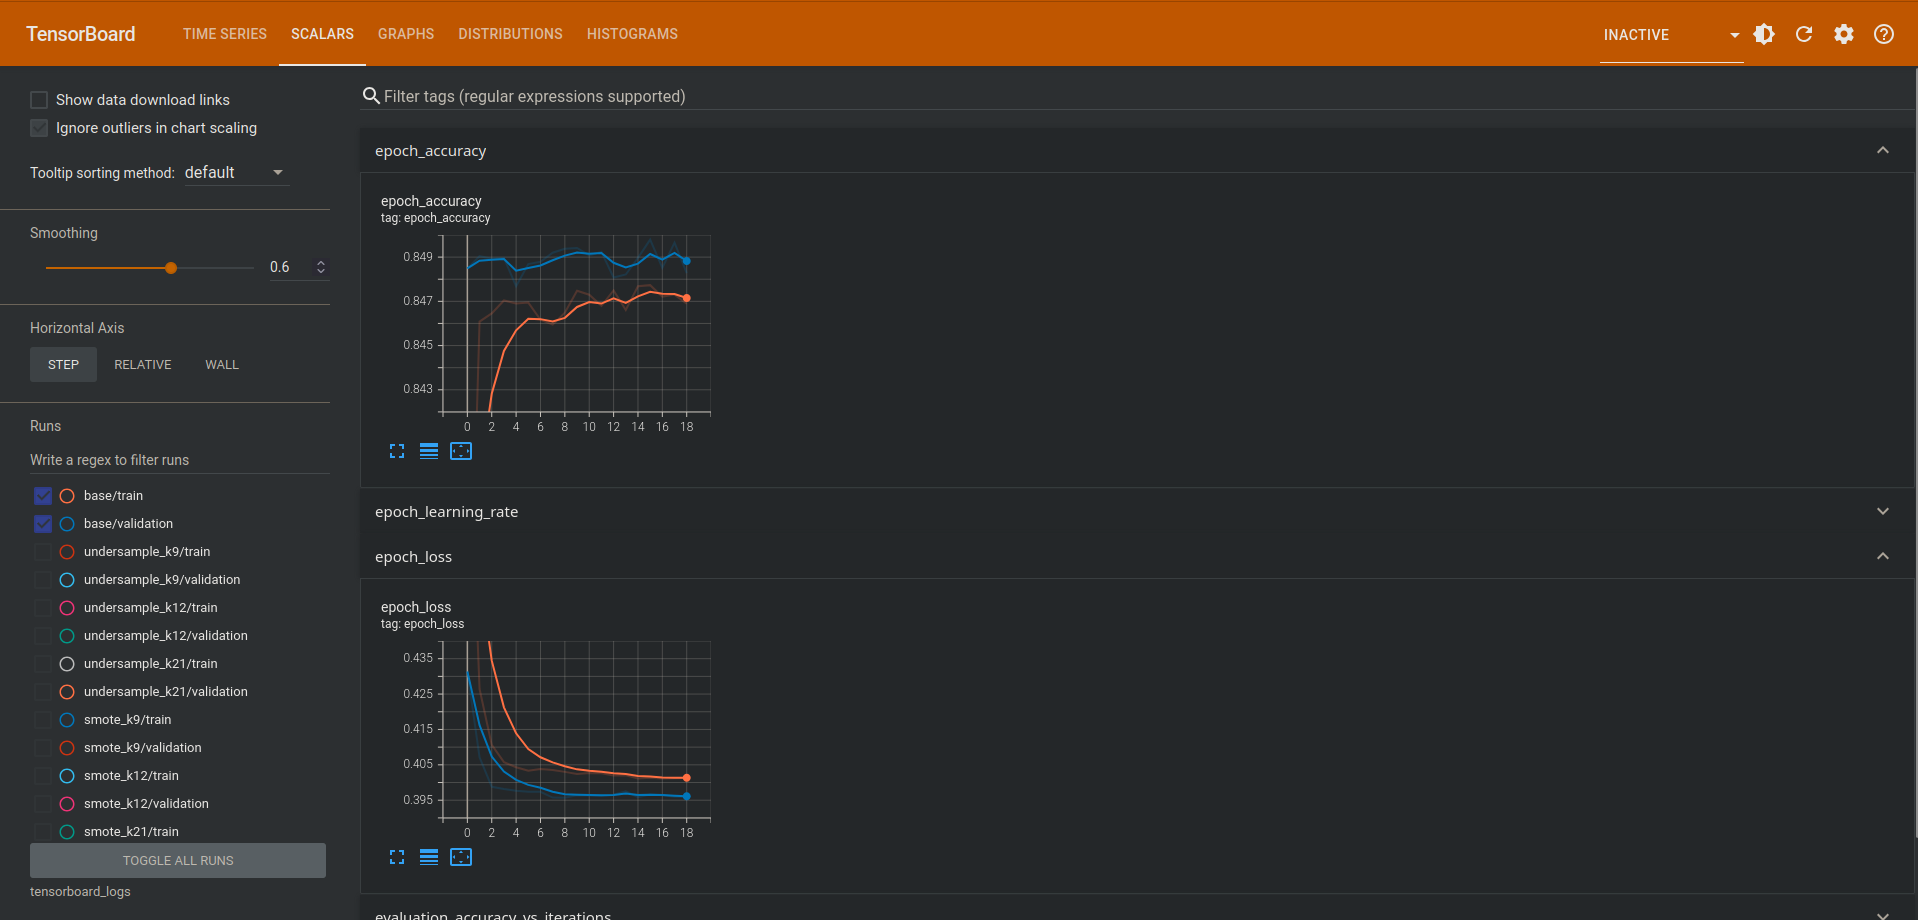
\includegraphics[width=1.1\textwidth,height=1.1\textwidth,keepaspectratio]{ts/1.png}
    \caption{Baseline TensorBoard}
\end{figure}
\vspace{1cm}
\hrule
\vspace{1cm}
\noindent\textbf{Observation:} The baseline run appears to have stable learning with no strong train-validation divergence, so severe overfitting is not obvious. However, relative to balanced runs, it likely underfits minority classes because optimization is dominated by the majority class.

\newpage
\begin{figure}[H]
    \hspace{-0.3cm}
    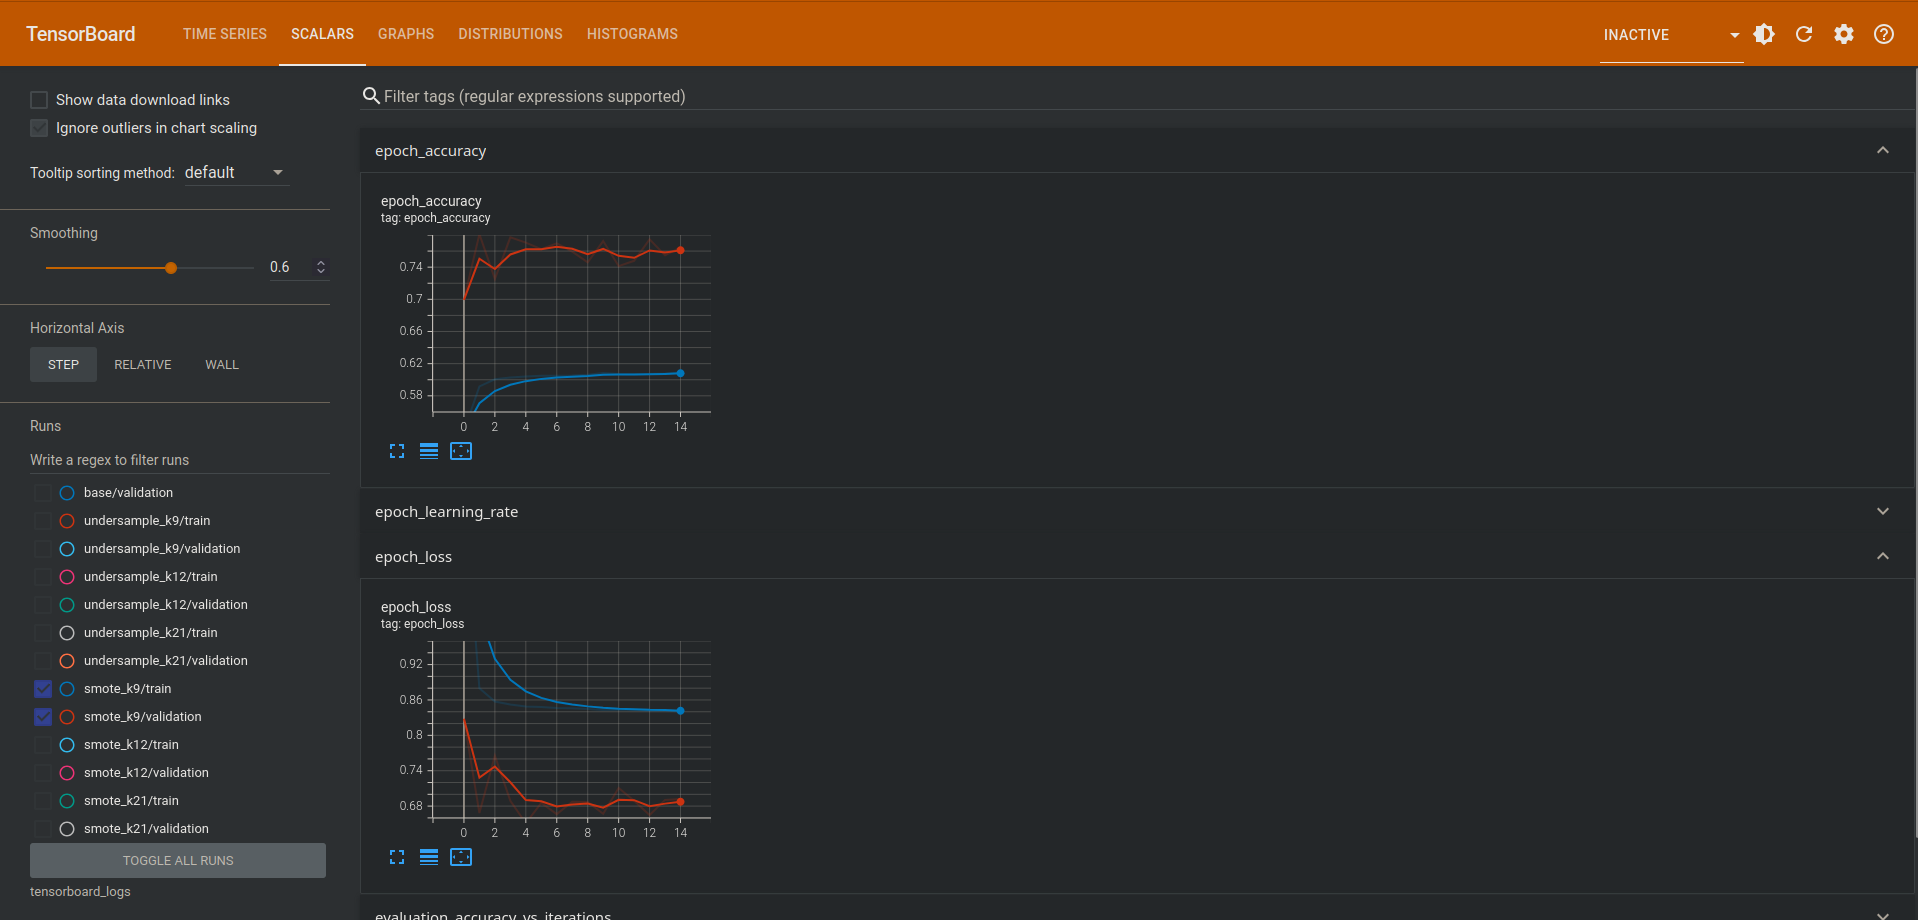
\includegraphics[width=1.1\textwidth,height=1.1\textwidth,keepaspectratio]{ts/2.png}
    \caption{SMOTE K=9 TensorBoard}
\end{figure}
\vspace{1cm}
\hrule
\vspace{1cm}
\noindent\textbf{Observation:} This run shows generally healthy convergence and only mild late-epoch gap behavior, suggesting limited overfitting. It looks better balanced than the baseline and does not show clear underfitting.

\newpage
\begin{figure}[H]
    \hspace{-0.3cm}
    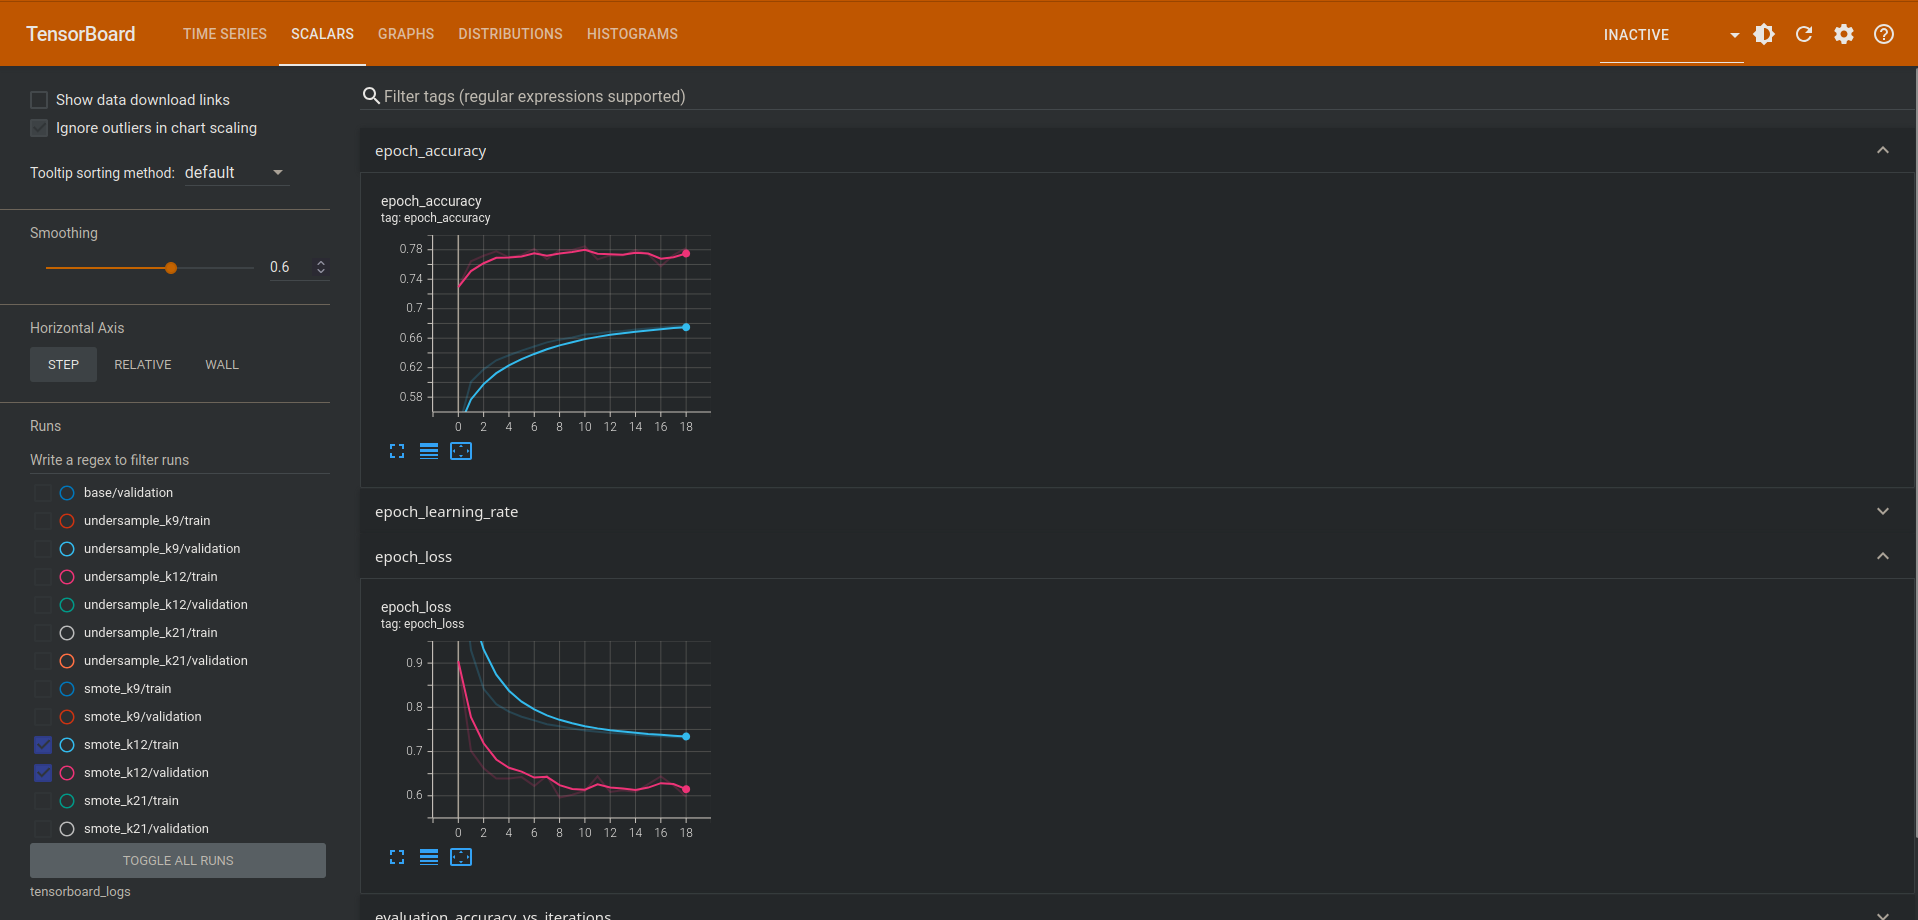
\includegraphics[width=1.1\textwidth,height=1.1\textwidth,keepaspectratio]{ts/3.png}
    \caption{SMOTE K=12 TensorBoard}
\end{figure}
\vspace{1cm}
\hrule
\vspace{1cm}
\noindent\textbf{Observation:} The curves are the most consistent among the SMOTE settings, with good validation tracking and no large persistent gap. This indicates the best trade-off here, with weak signs of overfitting and no meaningful underfitting.

\newpage
\begin{figure}[H]
    \hspace{-0.3cm}
    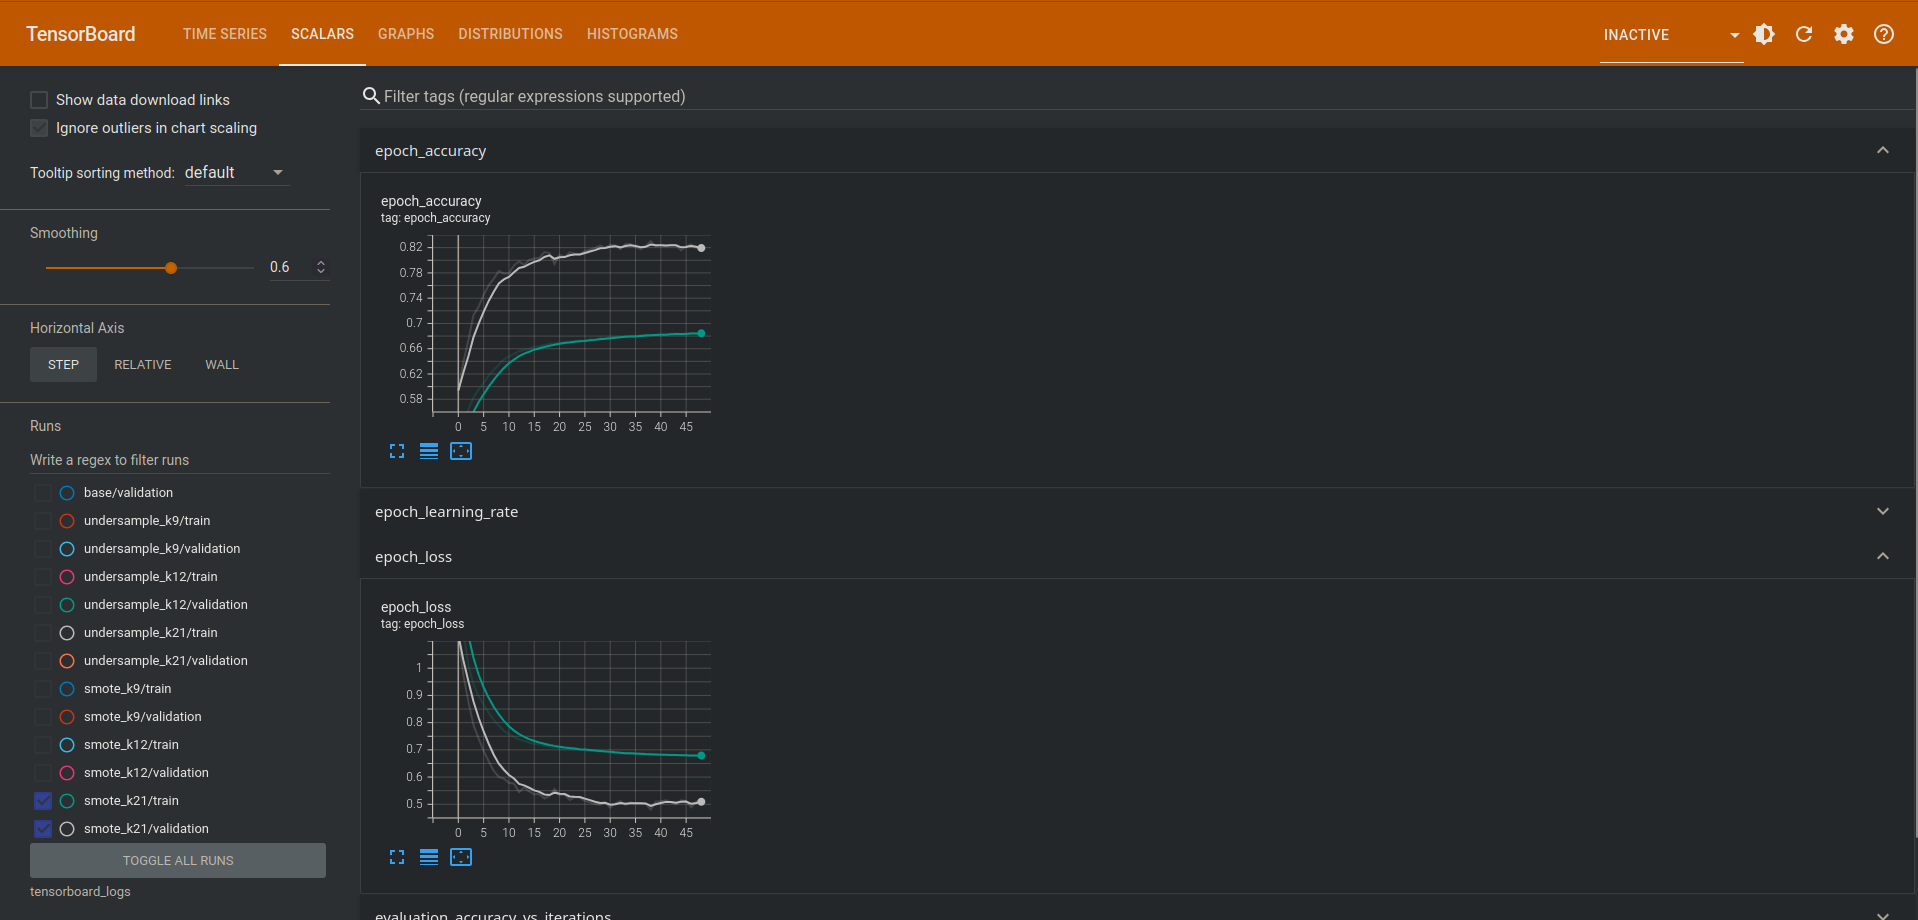
\includegraphics[width=1.1\textwidth,height=1.1\textwidth,keepaspectratio]{ts/4.png}
    \caption{SMOTE K=21 TensorBoard}
\end{figure}
\vspace{1cm}
\hrule
\vspace{1cm}
\noindent\textbf{Observation:} Compared with SMOTE $k=12$, this setting shows slightly weaker generalization behavior and a modest train-validation gap. That suggests mild overfitting pressure without clear severe underfitting.

\newpage
\begin{figure}[H]
    \hspace{-0.3cm}
    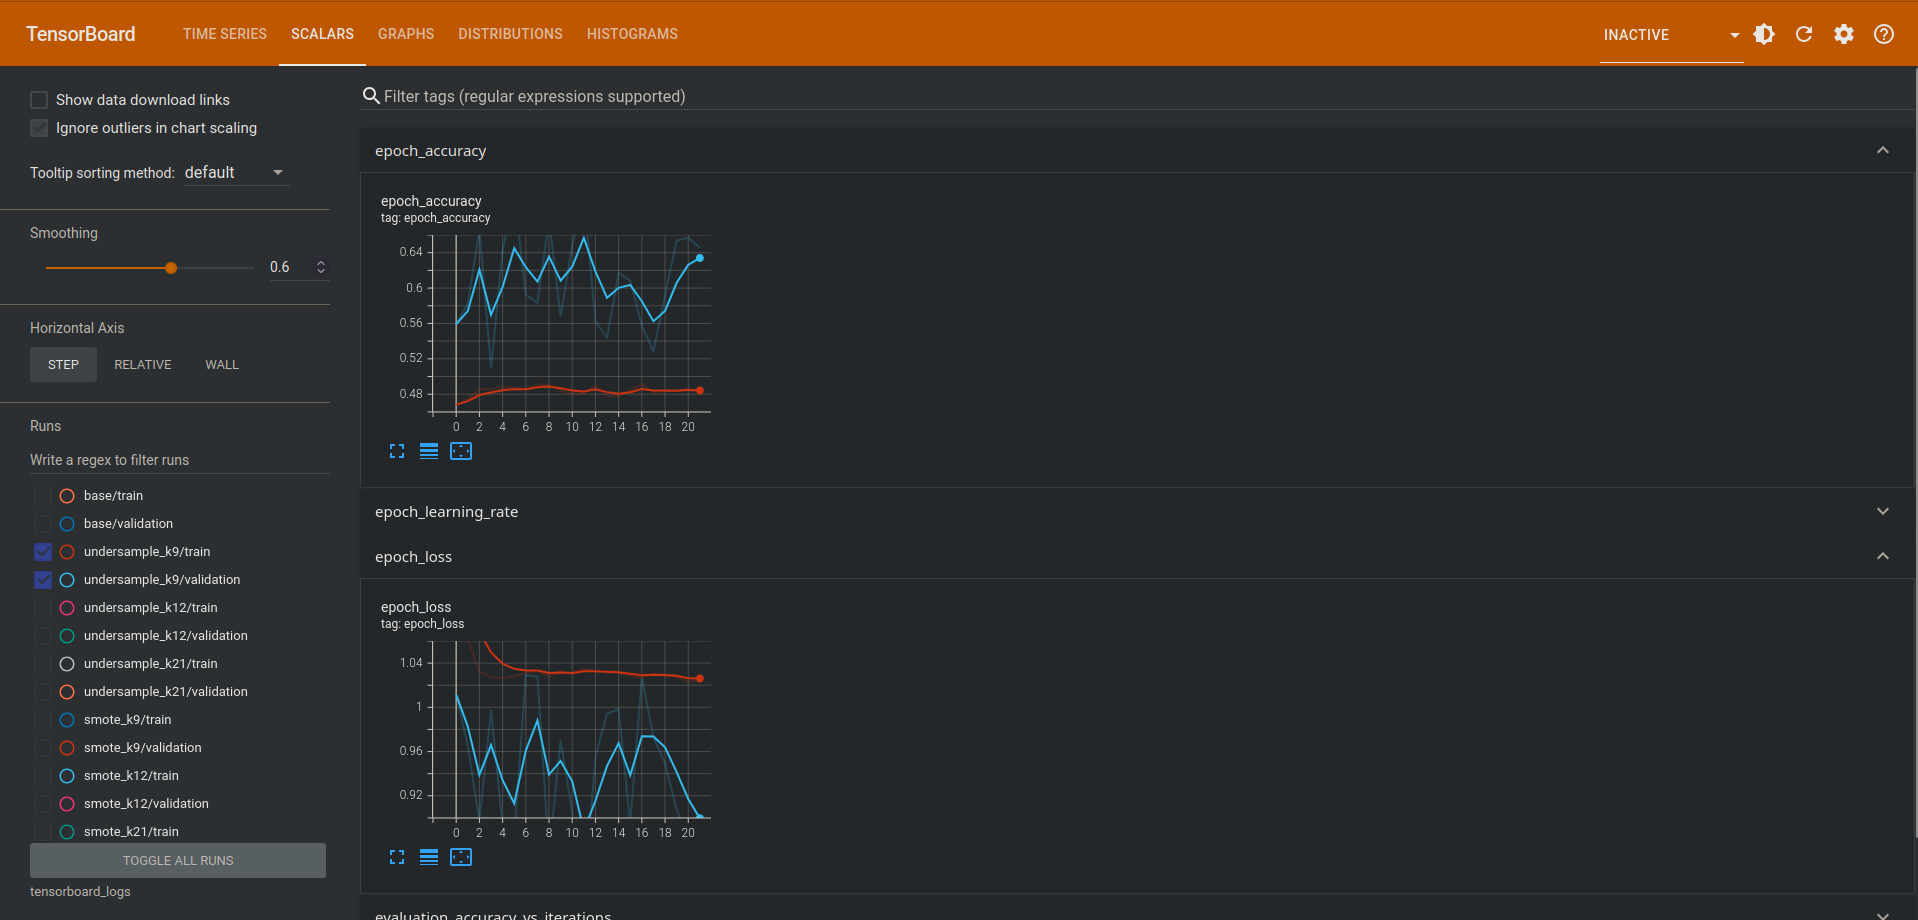
\includegraphics[width=1.1\textwidth,height=1.1\textwidth,keepaspectratio]{ts/5.png}
    \caption{Random Under-sampling K=9 TensorBoard}
\end{figure}
\vspace{1cm}
\hrule
\vspace{1cm}
\noindent\textbf{Observation:} Under-sampling at $k=9$ tends to converge quickly but to a lower performance ceiling, which is a typical sign of underfitting due to reduced training diversity. Overfitting is limited because the model capacity is effectively constrained by less data.

\newpage
\begin{figure}[H]
    \hspace{-0.3cm}
    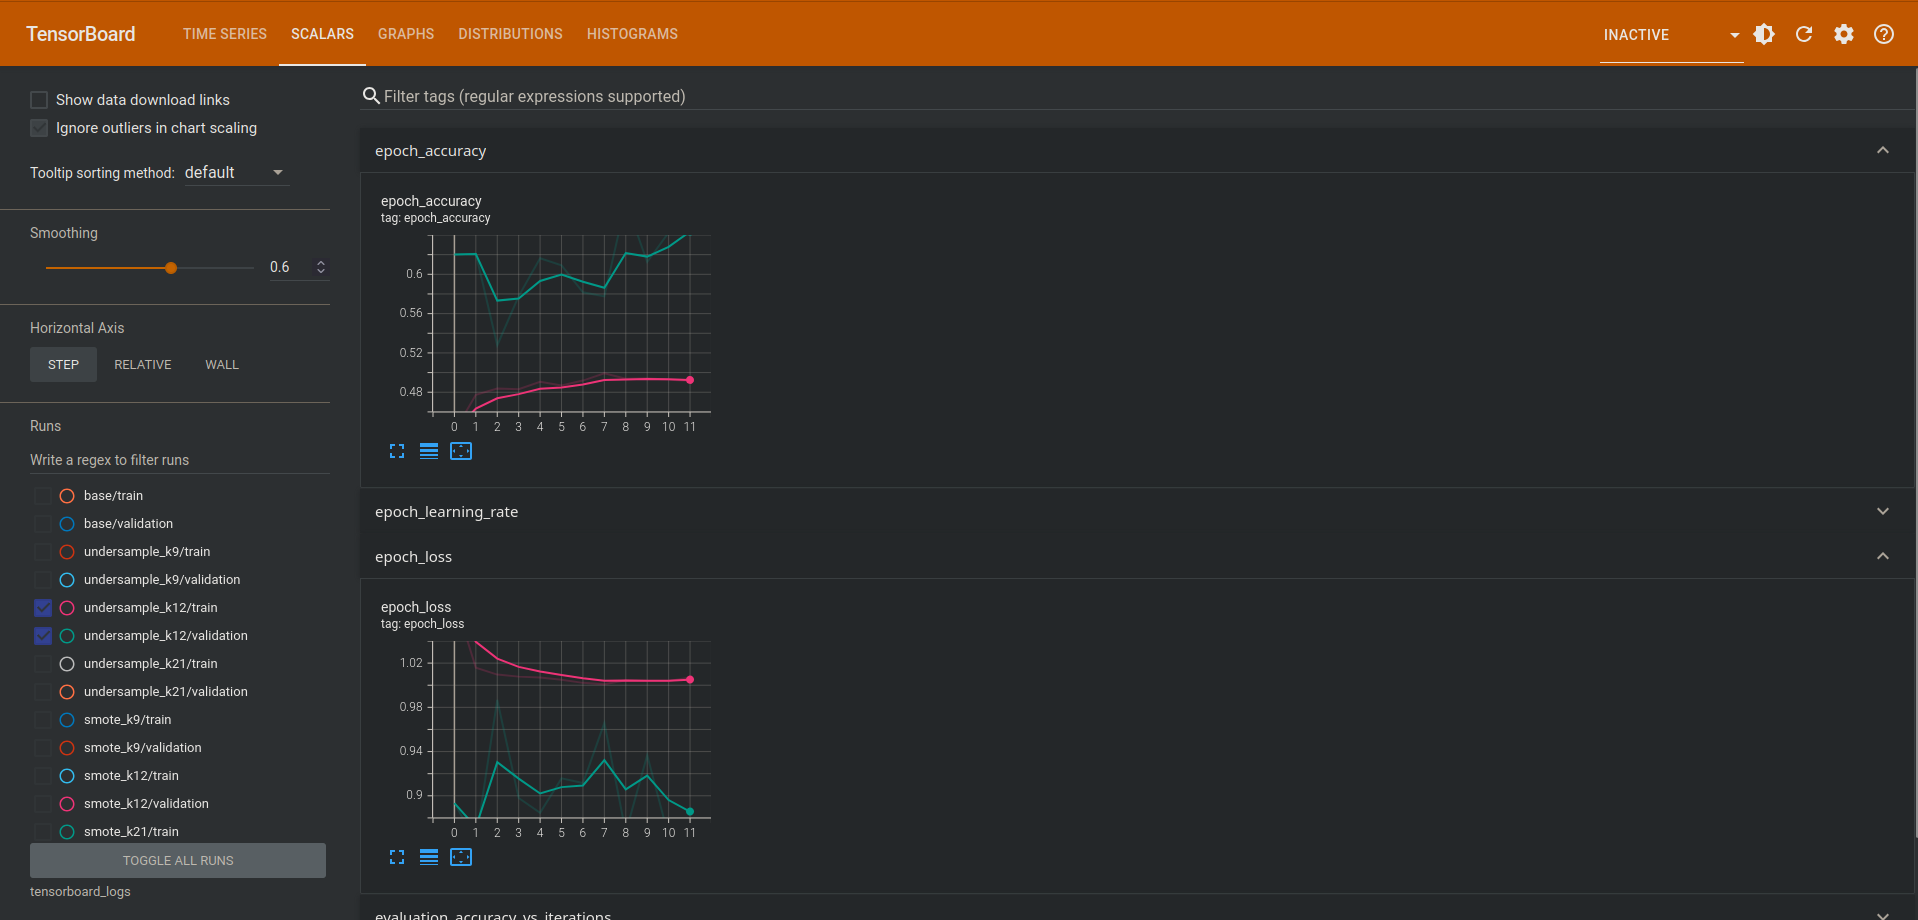
\includegraphics[width=1.1\textwidth,height=1.1\textwidth,keepaspectratio]{ts/6.png}
    \caption{Random Under-sampling K=12 TensorBoard}
\end{figure}
\vspace{1cm}
\hrule
\vspace{1cm}
\noindent\textbf{Observation:} This run shows the clearest underfitting tendency among the under-sampled settings, with validation improvement saturating early and weaker final performance. There is no strong evidence of classical overfitting.

\newpage 
\begin{figure}[H]
    \hspace{-0.3cm}
    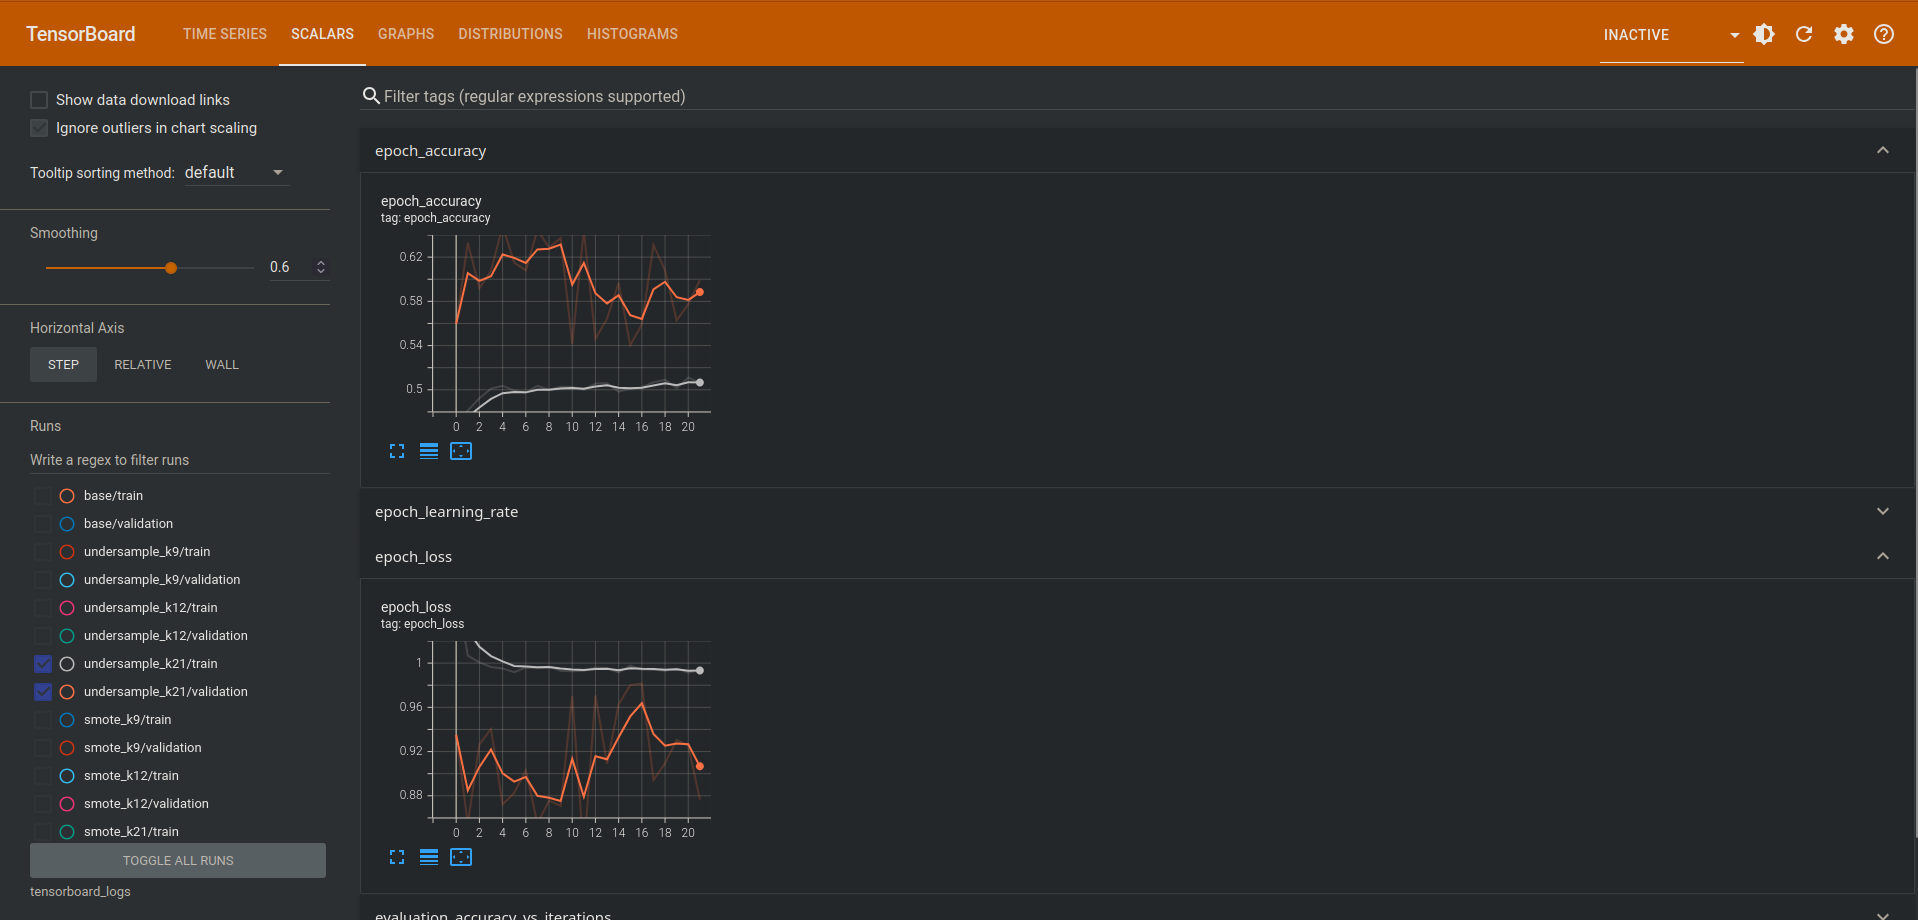
\includegraphics[width=1.1\textwidth,height=1.1\textwidth,keepaspectratio]{ts/7.png}
    \caption{Random Under-sampling K=21 TensorBoard}
\end{figure}
\vspace{1cm}
\hrule
\vspace{1cm}
\noindent\textbf{Observation:} The training dynamics are somewhat better than under-sampling $k=12$, but still suggest a constrained fit relative to SMOTE configurations. Overall this indicates mild-to-moderate underfitting with limited overfitting.


\newpage
\chapter{Evaluation Metrics}

\section{Comparison Strategy}
To compare the three model families fairly, we focus on four core metrics reported for all settings: \textbf{Accuracy}, \textbf{F1 Micro}, \textbf{F1 Macro}, and \textbf{F1 Weighted}. Accuracy and F1 Micro reflect overall correctness, while F1 Macro gives equal importance to all classes and is therefore more sensitive to minority-class performance.

\section{Baseline Comparison}
\begin{table}[H]
    \centering
    \caption{Baseline (Unbalanced Data) Comparison Across Model Families}
    \label{tab:baseline-comparison-all-models}
    \begin{tabular}{lcccc}
        \toprule
        \textbf{Model Family} & \textbf{Accuracy} & \textbf{F1 Micro} & \textbf{F1 Macro} & \textbf{F1 Weighted} \\
        \midrule
        KNN & 0.8219 & 0.8219 & 0.4016 & 0.7993 \\
        Softmax Regression & 0.8335 & 0.8335 & 0.3955 & 0.7931 \\
        Neural Network & 0.8493 & 0.8493 & 0.3898 & 0.8077 \\
        \bottomrule
    \end{tabular}
\end{table}

The baseline results show that the \textbf{Neural Network} obtains the highest overall performance (Accuracy/F1 Micro), while \textbf{KNN} provides a slightly stronger baseline \textbf{F1 Macro}. This indicates that the NN is best at global prediction correctness on the original distribution, but KNN is marginally more balanced across classes before rebalancing.

\section{Balanced Data Comparison (Shared Settings)}
\subsection{SMOTE Comparison}
\begin{table}[H]
    \centering
    \caption{SMOTE Comparison Across Model Families}
    \label{tab:smote-comparison-all-models}
    \begin{tabular}{llcccc}
        \toprule
        \textbf{Setting} & \textbf{Model Family} & \textbf{Accuracy} & \textbf{F1 Micro} & \textbf{F1 Macro} & \textbf{F1 Weighted} \\
        \midrule
        $k=9$ & KNN & 0.7298 & 0.7298 & 0.4276 & 0.7579 \\
        $k=9$ & Softmax & 0.6306 & 0.6306 & 0.4242 & 0.7032 \\
        $k=9$ & Neural Network & 0.7702 & 0.7702 & 0.4407 & 0.7818 \\
        \midrule
        $k=12$ & KNN & 0.7302 & 0.7302 & 0.4315 & 0.7592 \\
        $k=12$ & Softmax & 0.6289 & 0.6289 & 0.4221 & 0.7018 \\
        $k=12$ & Neural Network & 0.7819 & 0.7819 & 0.4468 & 0.7892 \\
        \midrule
        $k=21$ & Softmax & 0.6250 & 0.6250 & 0.4217 & 0.6998 \\
        $k=21$ & Neural Network & 0.8298 & 0.8298 & 0.4163 & 0.7999 \\
        \bottomrule
    \end{tabular}
\end{table}

Under SMOTE, the \textbf{Neural Network} gives the strongest Accuracy/F1 Micro in all reported settings and also achieves the best F1 Macro at $k=9$ and $k=12$. KNN remains competitive in macro performance at those settings, while Softmax is consistently lower across the four core metrics.

\subsection{Under-sampling Comparison}
\begin{table}[H]
    \centering
    \caption{Random Under-sampling Comparison Across Model Families}
    \label{tab:undersample-comparison-all-models}
    \begin{tabular}{llcccc}
        \toprule
        \textbf{Setting} & \textbf{Model Family} & \textbf{Accuracy} & \textbf{F1 Micro} & \textbf{F1 Macro} & \textbf{F1 Weighted} \\
        \midrule
        $k=9$ & KNN & 0.5870 & 0.5870 & 0.4020 & 0.6714 \\
        $k=9$ & Softmax & 0.6280 & 0.6280 & 0.4237 & 0.7019 \\
        $k=9$ & Neural Network & 0.7048 & 0.7048 & 0.4353 & 0.7431 \\
        \midrule
        $k=12$ & KNN & 0.5908 & 0.5908 & 0.4017 & 0.6735 \\
        $k=12$ & Softmax & 0.6263 & 0.6263 & 0.4222 & 0.7010 \\
        $k=12$ & Neural Network & 0.6216 & 0.6216 & 0.4173 & 0.6929 \\
        \midrule
        $k=21$ & Softmax & 0.6244 & 0.6244 & 0.4219 & 0.6996 \\
        $k=21$ & Neural Network & 0.6423 & 0.6423 & 0.4326 & 0.7162 \\
        \bottomrule
    \end{tabular}
\end{table}

For under-sampling, the Neural Network performs best at $k=9$ and $k=21$, but Softmax slightly surpasses it at $k=12$. KNN is consistently the weakest under under-sampling in this report, suggesting that aggressive class reduction harms neighborhood-based learning more than parametric models.

\section{Best Configurations by Objective}
\begin{table}[H]
    \centering
    \caption{Best Observed Configurations Across All Reported Results}
    \label{tab:best-overall-by-objective}
    \begin{tabular}{lll}
        \toprule
        \textbf{Objective} & \textbf{Best Configuration} & \textbf{Value} \\
        \midrule
        Highest Accuracy / F1 Micro & Neural Network (base) & 0.8493 \\
        Highest F1 Macro & Neural Network (smote\_k12) & 0.4468 \\
        Highest F1 Weighted & Neural Network (base) & 0.8077 \\
        \bottomrule
    \end{tabular}
\end{table}

Overall, the results indicate that \textbf{Neural Networks} provide the strongest performance envelope across both global and balanced metrics. \textbf{KNN} remains a viable baseline and can achieve competitive macro performance under SMOTE, while \textbf{Softmax Regression} is stable but generally trails in top-end performance. Therefore, model selection should follow the deployment goal: if maximum global accuracy is required, the NN baseline is preferred; if improved minority-class balance is prioritized, NN with SMOTE (especially $k=12$) is the best setting in this study.

\section{Best Evaluation Metric for Model Selection}
Given the class imbalance in the diabetes dataset, \textbf{F1 Macro} is the most appropriate metric for model selection in this context. It provides a balanced view of performance across all classes, ensuring that improvements in minority-class predictions are not overshadowed by the majority class. While Accuracy and F1 Micro can be misleading in imbalanced scenarios, F1 Macro offers a more nuanced assessment of how well the model performs across the entire class distribution, making it the best choice for selecting the most effective model for diabetes risk prediction in this study.



\newpage
\chapter{Discussion}
\section{Best Models}

\begin{table}[H]
    \centering
    \caption{Best Model per Algorithm (Selected by Highest F1 Macro)}
    \label{tab:best-model-per-algorithm}
    \begin{tabular}{llcccc}
        \toprule
        \textbf{Algorithm} & \textbf{Best Configuration} & \textbf{Accuracy} & \textbf{F1 Micro} & \textbf{F1 Macro} & \textbf{F1 Weighted} \\
        \midrule
        KNN & SMOTE ($k=12$) & 0.7302 & 0.7302 & 0.4315 & 0.7592 \\
        Softmax Regression & SMOTE ($k=9$) & 0.6306 & 0.6306 & 0.4242 & 0.7032 \\
        Neural Network & SMOTE ($k=12$) & 0.7819 & 0.7819 & 0.4468 & 0.7892 \\
        \bottomrule
    \end{tabular}
\end{table}

This summary highlights each algorithm's strongest configuration under the class-balance criterion used in this report (F1 Macro).

\subsection{Why These Were the Best Models}
The selected configuration for each algorithm is the one that achieved the highest \textbf{F1 Macro} within that algorithm's tested settings. This criterion is appropriate because the diabetes classes are imbalanced, so equal class-wise performance is more informative than accuracy alone.

For \textbf{KNN}, SMOTE ($k=12$) is best because it yields the top macro-level balance for KNN (\textbf{F1 Macro = 0.4315}) while preserving solid overall performance (Accuracy/F1 Micro = 0.7302).

For \textbf{Softmax Regression}, SMOTE ($k=9$) is best because it provides the strongest class-balanced Softmax result (\textbf{F1 Macro = 0.4242}) and is also the best Softmax setting by weighted F1 among the reported balanced variants.

For \textbf{Neural Networks}, SMOTE ($k=12$) is best because it achieves the highest macro performance not only within NN (\textbf{F1 Macro = 0.4468}) but also across all reported model families and settings, indicating the strongest minority-class handling.

\subsection{Comparison Between the Three Best Models}
Comparing the three best-per-algorithm models directly:
\begin{itemize}
    \item \textbf{Neural Network (SMOTE $k=12$)} outperforms \textbf{KNN (SMOTE $k=12$)} by +0.0517 Accuracy/F1 Micro, +0.0153 F1 Macro, and +0.0300 F1 Weighted.
    \item \textbf{Neural Network (SMOTE $k=12$)} outperforms \textbf{Softmax (SMOTE $k=9$)} by +0.1513 Accuracy/F1 Micro, +0.0226 F1 Macro, and +0.0860 F1 Weighted.
    \item \textbf{KNN (SMOTE $k=12$)} outperforms \textbf{Softmax (SMOTE $k=9$)} by +0.0996 Accuracy/F1 Micro, +0.0073 F1 Macro, and +0.0560 F1 Weighted.
\end{itemize}

Overall, the best NN model is the strongest in both global and balanced metrics, the best KNN model is second and remains reasonably competitive on F1 Macro, and the best Softmax model is the most conservative performer with the lowest scores among the three selected winners.


\newpage
\section{Imbalance Handling Effectiveness}
\begin{table}[H]
    \centering
    \small
    \caption{Imbalance-Handling Effectiveness by Algorithm (Macro-F1 Gain)}
    \label{tab:imbalance-effectiveness}
    \begin{tabular}{lccccc}
        \toprule
        \textbf{Algorithm} & \textbf{Baseline} & \textbf{Best Setting} & \textbf{Best Macro-F1} & \textbf{Gain} & \textbf{Gain (\%)} \\
        \midrule
        KNN & 0.4016 & SMOTE ($k=12$) & 0.4315 & +0.0299 & +7.44\% \\
        Softmax Regression & 0.3955 & SMOTE ($k=9$) & 0.4242 & +0.0287 & +7.26\% \\
        Neural Network & 0.3898 & SMOTE ($k=12$) & 0.4468 & +0.0570 & +14.62\% \\
        \bottomrule
    \end{tabular}
\end{table}

The effectiveness table shows that class-imbalance treatment improved Macro-F1 for all three algorithms. The Neural Network achieved the largest absolute and relative gain, indicating the strongest improvement in minority-class sensitivity after balancing.

\newpage
\section{Insights and Observations}
Analysis of the undersampling\_train\_k12 confusion matrix reveals significant misclassification patterns, particularly surrounding the minority "Prediabetes" class. Out of 926 true prediabetic cases, the model only identified 98 correctly, misclassifying 228 as "No Diabetes" and 600 as "Diabetes". Clinically, this occurs because prediabetes is a transitional state; without precise lab metrics (like A1C), the survey-based lifestyle features (BMI, HighBP) of a prediabetic patient heavily overlap with those of a diabetic patient. Mathematically, optimizing for Macro-F1 caused the Softmax decision boundaries to shift. Because the feature space for Class 1 is poorly defined and overlaps heavily with the other classes, the algorithm minimized its precision penalty by absorbing ambiguous cases into the broader "Diabetes" class. Additionally, the imbalance handling created a hypersensitive model, resulting in 9,485 healthy patients being falsely flagged as diabetic, illustrating the strict mathematical trade-off between minority class recall and majority class precision.

\end{document}